\documentclass[12pt]{article}

\usepackage{tikz}
\usetikzlibrary{calc}
\usetikzlibrary{shapes,arrows}
\usepackage{listings}
\usepackage[utf8]{inputenc}
\usepackage{graphicx}

\title{An Implementation of Halfedge Data Structure in Catmull-Clark 
Subdivision for 2-Manifold Single-sided Surface}
\author{Yu Wang}
\date{August 2015}

\makeatletter
\def\BState{\State\hskip-\ALG@thistlm}
\makeatother

\begin{document}
\maketitle
\newpage

%\begin{abstract} A place for abstract later
% Contents of abstract
%\end{abstract}
\tableofcontents
\newpage
\section{Introduction}
Many abstract geometrical sculptures have the shape of a (thickened) 2D surface embedded in 3D space. (Reference: 2-manifold sculpture). According to Surface Classification Theorem, All 2-manifolds (thin surfaces with borders) can be uniquely classified by their orientability (double-sided or single-sided), by the number b of their borders (loops of 1-dimensional rim lines), and their genus g (the number of independent closed loop cuts that can be made on such a surface, leaving all its pieces still connected to one another).

Researchers have developed multiple ways in order to build smooth surfaces with parametric initial inputs, including NURBS, Catmull-Clark subdivision and Loop subdivision. Catmull-Clark subdivision is widely applied to construct a smooth surface from an initial mesh of polygons. It is independent of the topology of initial mesh.

When working with Berkeley SLIDE Environment (Reference: http://www.cs.berkeley.edu/~ug/slide/), an issue of Catmull-Clark Subdivision occurs. The subdivision result breaks apart at Mobius connection of the geometry. In order to address this issue, we developed a machine that uses an extended definition of halfedge data structure to generate Catmull-Clark subdivsion and offset for single-sided surfaces.

\newpage
\section{Halfedge Data Structure} \label{sec:halfedge}

An object in the 3D Euclid space can be modeled as several meshes of polygons. For a single mesh, it comprises three types of geometry elements: vertex, edge, and face. Adjacency data structure is need to store the topological information (adjacency and connectivity) between these elements.

Several adjacency structures have been fully developed, including simple data structure, winged edge data structure (Baumgart, 1975), halfedge data structure (Eastman, 1982), QuadEdge Data structure (Guibas and Stolfi), and FaceEdge Data Structure (Dobkin and Laszlo, 1987).

Among all these data structures, the author chooses halfedge data structure in this project to realize Catmull-Clark subdivision, because 1) the storage size is independent of the mesh topology, and 2) it has a simple implementation. The author also extends its definition to add the ability in dealing with single-sided surfaces (or non-orientable object).

\subsection{Vertex, Halfedge, and Face}

The definitions and assumptions of vertex, halfedge and face follow the assumption of 2-manifold, as shown in Table \ref{table:vhfdef}. Element IDs are unique. When two elements fall into the same group of element, they can not have same ID. (Mobius sibling halfedges are exceptions as we discuss later). A quadrilateral face made with four halfedges and four vertices is shown in Figure \ref{figure:singleFace}.

%Table1
\begin{table}[h]
\centering
\begin{tabular}{| l | p{0.4\textwidth} | p{0.4\textwidth}|}

\hline
		&	Definition	& Assumption	\\
\hline
Vertex	&	A 3-dimensional point.		&	No overlapping vertices exits in a mesh. But overlapping vertices can exist in different meshes.\\
\hline
Halfedge	&	An edge that starts from one vertex and ends at another vertex. & A halfedge connects exactly two non-overlapping vertices and it has a direction. 
Less than two halfedges start from the same vertex and end at the same vertex in a single mesh.\\
\hline
Face		&	A polygon that contains a loop of vertices and halfedges.	& A face has at least three non-overlapping vertices so it makes a polygon. The face has to be constructed with a complete loop of halfedges with on openings.\\
\hline
\end{tabular}
\caption{Definitions and assumptions of vertex, halfedge, and face} 
\label{table:vhfdef}
\end{table}

%Figure1
\begin{figure}[h]
  \centering
  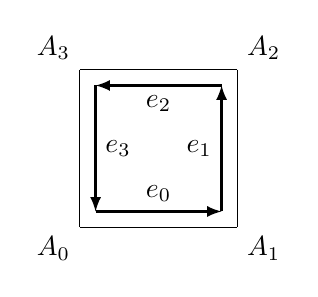
\begin{tikzpicture}
    \coordinate (A0) at (0,0);
    \coordinate (A1) at (2,0);
    \coordinate (A2) at (2,2);
    \coordinate (A3) at (0,2);
    \coordinate (B0) at (0.2,0.2);
    \coordinate (B1) at (1.8,0.2);
    \coordinate (B2) at (1.8,1.8);
    \coordinate (B3) at (0.2,1.8);
      \draw(A0)
        -- (A1) node [below right] {$A_1$};
      \draw (A1)
        -- (A2) node [above right] {$A_2$};
      \draw (A2)
        -- (A3) node [above left] {$A_3$};
      \draw (A3)
        -- (A0) node [below left] {$A_0$};
      \draw  [thick,-latex] (B0)
        -- (B1);
      \draw [thick,-latex,] (B1)
        -- (B2);
      \draw [thick,-latex,] (B2)
        -- (B3);
      \draw [thick,-latex,] (B3)
        -- (B0);
      \node [right] at (0.2, 1) {$e_3$};
      \node [above] at (1, 0.2) {$e_0$};
      \node [left] at (1.8, 1) {$e_1$};
      \node [below] at (1, 1.8) {$e_2$};
  \end{tikzpicture}
  \caption{A quadrilateral face made with four halfedges}
  \label{figure:singleFace}
\end{figure}

Every element stores two types of information: self-information and adjacency information. As shown in Table \ref{table:vhfInfo}. The adjacency information includes adjacency in a face and adjacency between faces. The adjacency between faces include sibling links and boundary links. (And we will discussion more in the mesh section.) 

%Table2
\begin{table}[ht]
\centering
\begin{tabular}{| l | p{0.4\textwidth} | p{0.4\textwidth}|}

\hline
Element & Self-Information & Adjacency Information  \\
\hline
Vertex  & 1. vertex ID & 1. one outgoing halfedge   \\
& 2. vertex position & 2. mobius indicator \\
& 3. vertex normal & \\
\hline
Halfedge & 1. edge ID & 1. start and end vertex\\
& & 2. link to parent face\\
& & 3. predecessor and successor in the parent face\\
& & 4. sibling links to adjacent face\\
& & 5. boundary links to adjacent face \\
\hline
Face    &  1. face ID & 1. one side halfedge\\
& 2. face normal &\\
\hline
\end{tabular}
\caption{Definitions and assumptions of vertex, halfedge, and face} 
\label{table:vhfInfo}
\end{table}

\subsection{Mesh}
We define a mesh as a collection of basic elements (i.e. vertex, halfedge, and face). Hashtable is implemented to represent the collection in this project, because of its constant serach time for element. We construct three hashtables for all vertices, halfedges, and faces in the mesh respectively. The keys for these hashtable are element IDs and the contents are the element pointers.

The ID of a halfedge is related with the IDs of its start vertex and end vertex. In this project, we define the ID of a halfedge as start vertex ID * maximum number of vertices in a mesh + end vertex ID. This definition will guarantee a unique ID for every halfedge when they have a different start or different end vertex from other halfedges. 

A mesh also includes the adjacency and connectivity for elements within. They can be classified into three groups: 1) halfedge flow in a single face, 2) face connections, and 3) boundary connections.

\subsubsection{Halfedge Flow in a Single Face}
A face is constructed by a loop of consecutive halfedges. The start of one halfedge is the end of its previous halfedge, and the end is the start of its next halfedge. Every halfedge contains two pointers, pointing to its previous and next halfedge respectively. Every vertex in this face will also have a pointer to its outgoing halfedge.

\subsubsection{Face Connections and Sibling Links}

There are two types of face connections, the normal connection and the mobius connection, as shown in Figure \ref{figure:faceConnections}. In a typical halfedge data structure, with the assumption of double-sided surface, a pair of halfedges between two faces is defined with opposite direction. We extends this idea to represent single-sided surface by adding another type of connection, named as mobius connection. In a mobius connection, a pair of halfedges are in same direction. The vertex on a mobius connection will also be marked for the purpose of vertex traversal in the future. In the example of Figure \ref{figure:faceConnections}, on the top, $e_1$ and $e_1'$ are siblings to each other. On the bottom, $e_1$ and $e_1'$ are mobius siblings to each other. 

One thing to point out is that mobius sibling halfedges have the same element ID. Because they have the same start vertex and end vertex. However, we could check for the mobius sibling pointers in order to find all halfedges in the edge traversal of a mesh.

With the extension of mobius connection, there can be three different adjacent situations for a halfedge in a mesh: 1) it is on a normal connection and has a normal sibling, 2) it is on a mobius connection and has a mobius pointer, and 3) it lies on the boundary of the surface and does not have a sibling pointer nor a mobius pointer.

%Figure2
\begin{figure}[ht]
  \centering
  %Normal Junction
  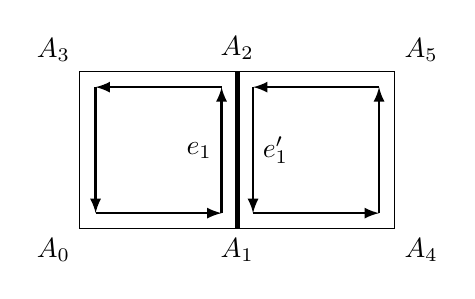
\begin{tikzpicture}
    \coordinate (A0) at (0,0);
    \coordinate (A1) at (2,0);
    \coordinate (A2) at (2,2);
    \coordinate (A3) at (0,2);
    \coordinate (A4) at (4,0);
    \coordinate (A5) at (4,2);
    \coordinate (B0) at (0.2,0.2);
    \coordinate (B1) at (1.8,0.2);
    \coordinate (B2) at (1.8,1.8);
    \coordinate (B3) at (0.2,1.8);
    \coordinate (B4) at (2.2,0.2);
    \coordinate (B5) at (3.8,0.2);
    \coordinate (B6) at (3.8,1.8);
    \coordinate (B7) at (2.2,1.8);
      \draw(A0) -- (A1) node [below] {$A_1$};
      \draw [ultra thick] (A1) -- (A2) node [above] {$A_2$};
      \draw (A2) -- (A3) node [above left] {$A_3$};
      \draw (A3) -- (A0) node [below left] {$A_0$};
      \draw (A1) -- (A4) node [below right] {$A_4$};
      \draw (A4) -- (A5) node [above right] {$A_5$};
      \draw (A5) -- (A2);
      \draw  [thick,-latex] (B0)
        -- (B1);
      \draw [thick,-latex,] (B1)
        -- (B2);
      \draw [thick,-latex,] (B2)
        -- (B3);
      \draw [thick,-latex,] (B3)
        -- (B0);
      \draw  [thick,-latex] (B4)
        -- (B5);
      \draw [thick,-latex,] (B5)
        -- (B6);
      \draw [thick,-latex,] (B6)
        -- (B7);
      \draw [thick,-latex,] (B7)
        -- (B4);
      \node [left] at (1.8, 1) {$e_1$};
      \node [right] at (2.2, 1) {$e_1'$};
  \end{tikzpicture}
  
  %Mobius Junction
  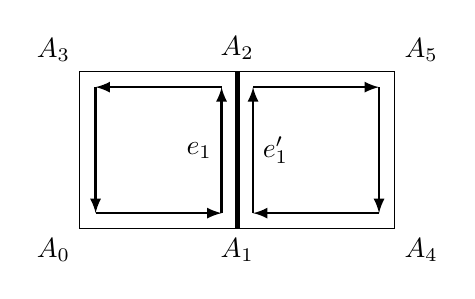
\begin{tikzpicture}
    \coordinate (A0) at (0,0);
    \coordinate (A1) at (2,0);
    \coordinate (A2) at (2,2);
    \coordinate (A3) at (0,2);
    \coordinate (A4) at (4,0);
    \coordinate (A5) at (4,2);
    \coordinate (B0) at (0.2,0.2);
    \coordinate (B1) at (1.8,0.2);
    \coordinate (B2) at (1.8,1.8);
    \coordinate (B3) at (0.2,1.8);
    \coordinate (B4) at (2.2,0.2);
    \coordinate (B5) at (3.8,0.2);
    \coordinate (B6) at (3.8,1.8);
    \coordinate (B7) at (2.2,1.8);
      \draw(A0) -- (A1) node [below] {$A_1$};
      \draw [ultra thick] (A1) -- (A2) node [above] {$A_2$};
      \draw (A2) -- (A3) node [above left] {$A_3$};
      \draw (A3) -- (A0) node [below left] {$A_0$};
      \draw (A1) -- (A4) node [below right] {$A_4$};
      \draw (A4) -- (A5) node [above right] {$A_5$};
      \draw (A5) -- (A2);
      \draw  [thick,-latex] (B0)
        -- (B1);
      \draw [thick,-latex,] (B1)
        -- (B2);
      \draw [thick,-latex,] (B2)
        -- (B3);
      \draw [thick,-latex,] (B3)
        -- (B0);
      \draw  [thick,-latex] (B5)
        -- (B4);
      \draw [thick,-latex,] (B4)
        -- (B7);
      \draw [thick,-latex,] (B7)
        -- (B6);
      \draw [thick,-latex,] (B6)
        -- (B5);
      \node [left] at (1.8, 1) {$e_1$};
      \node [right] at (2.2, 1) {$e_1'$};
  \end{tikzpicture}
  \caption{Normal connection (up) and mobius connection (down) between two faces}
  \label{figure:faceConnections}
\end{figure}

\subsubsection{Boundary and Boundary Links}

For halfedges on the boundary of a mesh, we connect them with boundary links. In a surface with no mobius connection, the boundary halfedges follow a continuous flow. We can traverse the boundary when starting at one vertex, following the natural flow on the boundary, and ending at the starting vertex. Previous boundary pointers and next boundary pointers are created to link these halfedges. When mobius connection occurs in a mesh, however, some adjacent boundary halfedges will start or end at same vertex, which blocks the natural flow of boundary halfedges. If this happens, we build mobius boundary pointers to link these halfedges. Figure X shows an example of boundary halfedges with and without mobius connections.

<Add normal boundary links figure and mobius boundary link figures here!>

\subsubsection{Build Mesh from Elements}

As a conclusion of adjacency in a mesh, we need four steps in order to construct a mesh from basic elements.

Step 1: Create individual vertices. We create instances of vertices with their position and ID. The position of two vertices can be the same but their ID should always be unique. 

This step takes O(V) time, where V is the number of vertices in the mesh.

Step 2: Construct individual faces. To build an individual face, we create consecutive instances of halfedges, with their start and end vertices. Meanwhile, every vertex will be assigned a pointer to its outgoing halfedge when we create halfedges. For each halfedge, We then add the previous and next pointers to its previous halfedge and next halfedge respectively. 

This step takes O(E) time, where E is the number of halfedges in the mesh.

Step 3: Build sibling links. For every halfedge, we need to find if there exist a sibling or mobius sibling from other faces in this mesh. If its start vertex is same with the end of another halfedge, and its end vertex is same with the start of another halfedge, we then find a sibling. If it has the same start and end vertex with another halfedge, we then find a mobius sibling. 

In this project, with the implementation of hashtable, the ID of a halfedge is related with its start vertex ID and end vertex ID. The mobius sibling link is actually generated in step 2. When we create the halfedge, if its ID is equal to a halfedge that we created before, we know they are mobius siblings. The search of normal sibling is also in constant time because we can calculate the ID of its sibling halfedge knowing that start and end vertex are reversed. 

This step takes O(E) time, where E is number of halfedges in the mesh.

Step 4: Build boundary links. After step 3, if a halfedge does not have a sibling or mobius sibling, it lies on the boundary of this mesh. We need to build the boundary links to these halfedges.

To do this, we need a counter to keep track of how many times we cross a mobius connection. We 1) set counter equal to zero and start from one halfedge on the boundary, 2) we go to its next halfedge if the counter is even, or its previous halfedge if the counter is odd, 3) we then go to its the sibling or moibus sibling, the counter increase by 1 if it is a mobius sibling, 4) check if the current halfedge is on boundary, if not, we repeat 2) and 3) until we reach to one, and 5) this boundary halfedge shares one vertex with our last boundary halfedge, so we can build boundary links between them, and 6) we repeat 1) to 5) to build bounary links until we reach the starting boundary halfedge in 1). From 1) to 6), one boundary loop of this mesh is built. And we move on to build other loops by repeating 1) to 6), until every boundary halfedges have boundary links to its adjacent boundaries.

This step takes O(E) time, where E is the number of halfedges in the mesh.

Now this mesh contains everything that we need to start a Catmull-Clark subdivision. In total, it takes O(E) time from step 1 to step 4.

\subsection{Mesh Operations}
Building from basic elements is not the only way to create the initial mesh for Catmull-Clark subdivison. A new mesh can also be made by the following mesh operations: 1) copy a mesh, 2) 3D transformation of a mesh, and 3) merging the boundaries for two meshes. 

\subsubsection{Copy a Mesh}
In order to make a copy, we create one element instance for every element that belongs to the original mesh. The copy of a mesh will keep the adjacency for elements and positions of vertices. Therefore, new element instances remain exact same adjacency information as the original mesh, except that the element ID is different and pointers are pointing to the new instances. 

\subsubsection{Mesh Transformation}
In a 3D transformation, the positions for all vertices in the mesh will perform transformation. The adjacency of original mesh remains the same, so halfedges and faces will transform at the same time while vertices transform. Typically, for linear transformations, we multiply the transformation matrix to the position of every vertex from the original mesh.

\subsubsection{Merging Meshes}
Meshes can be merged into a new mesh if sibling links can be made between some of the boundary halfedges that belongs them. This merge of boundary halfedge will keep the new mesh as a 2-manifold. We also want the elements ID from these meshes stays different, so no collision occurs after we merge them together.

Two types of mesh merging are implemented in this project: automatic merging and manual merging. In automatic merging, we define a very small tolerance value. If any pair of vertices on the boundary of the two meshes has a distance smaller than the tolerance, we check if their boundary halfedges can be merged with sibling links. If they do, we merge them, continue to trace along the boundaries of these two meshes and merge boundary halfedges until we can't.

In manual merging, we force to merge boundaries from two meshes even if the distance of their vertices are larger than tolerance. In practice, we have four ways to perform the manual merging. Assume we would like to force merge the boundary of Mesh 1 and Mesh 2, we can apply one of the following strategies:

1) Vertex positions in mesh 1 remain the same after merging. The boundary faces on Mesh 2 extend to the boundary of Mesh 1.

2) The opposite of 1).

3) Use the arithmetic mean position for vertex from Mesh 1 and Mesh 2 as the final vertex position after merging. The boundary faces from Mesh 1 and Mesh 2 both extend to these new vertex positions.

4) Build new faces between the two meshes and the vertex positions for Mesh 1 and Mesh 2 remain the same.

\subsection{Mesh Traversals} 
Catmull-Clark subdivision also requires two types of traversals in a mesh: 1) traversal around a face, and 2) traversal around a vertex. Traversal around a face is necessary to build face points and calculate face normal in the face. Traversal around a vertex is necessary to build vertex points and calculate vertex normal in the face.

\subsubsection{Traversal Around Face}
The traversal around a face lead to all the edges and vertices belong to this face. It starts from one side halfedge of this face, follows the halfedge flow, and ends at starting the halfedge of the traversal.
Traversals of all faces in a mesh takes O(E) time, where E is the number of faces in the mesh.

\subsubsection{Traversal Around Vertex}
The traversal around a vertex leads to all edges and faces that contain this vertex. The traversal of a vertex need to consider two issues: 1) is this vertex on a boundary, and  2) is this vertex on a mobius connection. This makes four different types of vertex traversals. See Figure \ref{figure:traversalAroundVertexNormal} - \ref{figure:traversalAroundVertexMobiusB} for examples.

In the vertex traversal without boundary and mobius issue, we start from one outgoing halfedge of this vertex. We continue to go to the next outgoing halfedge by going to the successor of its sibling until we hit the first outgoing halfedge. In the example of Figure \ref{figure:traversalAroundVertexNormal}, if start and end at halfedge $e_1$, the sequence of traversal is: $e_1$ (sibling link to) $e_1'$ (successor link to) $e_2$ (sibling link to) $e_2'$ (successor link to) $e_3$ (sibling link to) $e_3'$ (successor link to) $e_4$ (sibling link to ) $e_4'$  (successor link to)  $e_1$.

In order to address the issue of a vertex on boundary, instead of using sibling links, we use boundary links. In the example of Figure \ref{figure:traversalAroundVertexNormalB}, we have a boundary $e_4'$ to $e_2$. If start and end at halfedge $e_1$, the sequence of traversal is: $e_1$ (sibling link to) $e_1'$ (successor link to) $e_2$ (boundary link to) $e_4'$ (successor link to)  $e_1$.

To address the issue of vertex on a mobius connection, instead of using normal links, we use mobius links. At the same time, we switch between the successor and predecessor to the sibling every time we hit a mobius connection.  In the example of Figure \ref{figure:traversalAroundVertexNormal}, $e_1$ to $e_1'$ and $e_3$ to $e_3'$ have mobius siblings rather than normal sibling. If start and end at halfedge $e_1$, the sequence of traversal is: $e_1$ (mobius sibling link to) $e_1'$ (predecessor link to) $e_2$ (sibling link to) $e_2'$ (predecessor link to) $e_3$ (mobius sibling link to) $e_3'$ (successor link to) $e_4$ (sibling link to ) $e_4'$  (successor link to)  $e_1$.

If boundary and mobius connection both occur, we use a combination of the two methods above. In the example of Figure \ref{figure:traversalAroundVertexNormal}, $e_1$ to $e_1'$ and $e_3$ to $e_3'$ have mobius siblings rather than normal sibling and we have a mobius boundary connection between $e_4'$ and $e_2$. If starting and ending at halfedge $e_1$, the sequence of traversal is: $e_1$ (mobius sibling link to) $e_1'$ (predecessor link to) $e_2$ (mobius boundary link to ) $e_4'$  (successor link to)  $e_1$.

As a summary of the four different situations above, in a vertex traversal, we 1) start the traversal from with one outgoing halfedge of the vertex, 2) go to sibling or boundary link halfedge, 3) go to the next or previous halfedge that contains the vertex as one end, and 4) repeat 2) and 3) until we reach to the starting outgoing halfedge. This vertex traversal runs in O(E) time, where E is the total number of halfedges in the mesh.

%Figure3
\begin{figure}[ht]
  \centering
  %Normal Junction
  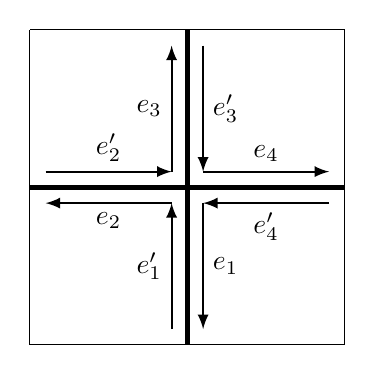
\begin{tikzpicture}
    \coordinate (A0) at (0,0);
    \coordinate (A1) at (2,0);
    \coordinate (A2) at (2,2);
    \coordinate (A3) at (0,2);
    \coordinate (A4) at (4,0);
    \coordinate (A5) at (4,2);
    \coordinate (A6) at (4,4);
    \coordinate (A7) at (2,4);
    \coordinate (A8) at (0,4);
    
    \coordinate (B0) at (0.2,0.2);
    \coordinate (B1) at (1.8,0.2);
    \coordinate (B2) at (1.8,1.8);
    \coordinate (B3) at (0.2,1.8);
    \coordinate (B4) at (2.2,0.2);
    \coordinate (B5) at (3.8,0.2);
    \coordinate (B6) at (3.8,1.8);
    \coordinate (B7) at (2.2,1.8);
    \coordinate (B8) at (0.2,2.2);
    \coordinate (B9) at (1.8,2.2);
    \coordinate (B10) at (1.8,3.8);
    \coordinate (B11) at (0.2,3.8);
    \coordinate (B12) at (2.2,2.2);
    \coordinate (B13) at (3.8,2.2);
    \coordinate (B14) at (3.8,3.8);
    \coordinate (B15) at (2.2,3.8);

     \draw (A0) -- (A1);
     \draw [ultra thick](A1) -- (A2);
     \draw  [ultra thick](A2) -- (A3);
     \draw (A3) -- (A0);
     \draw (A1) -- (A4);
     \draw (A4) -- (A5);
     \draw [ultra thick](A5) -- (A2);
     \draw (A3) -- (A8);
     \draw (A8) -- (A7);
     \draw (A7) -- (A6);
     \draw (A6) -- (A5);
     \draw [ultra thick] (A7) -- (A2);

     \draw [thick,-latex,] (B1) -- (B2);
     \draw [thick,-latex,] (B2) -- (B3);
     \draw [thick,-latex,] (B6) -- (B7);
     \draw [thick,-latex,] (B7) -- (B4);
     \draw [thick,-latex,] (B8) -- (B9);
     \draw  [thick,-latex] (B9) -- (B10);
     \draw [thick,-latex,] (B15) -- (B12);
     \draw [thick,-latex,] (B12) -- (B13);
     \node [left] at (1.8, 1) {$e_1'$};
     \node [right] at (2.2, 1) {$e_1$};
     \node [left] at (1.8, 3) {$e_3$};
     \node [right] at (2.2, 3) {$e_3'$};
     \node [below] at (1, 1.8) {$e_2$};
     \node [above] at (1, 2.2) {$e_2'$};
     \node [below] at (3, 1.8) {$e_4'$};
     \node [above] at (3, 2.2) {$e_4$};
  \end{tikzpicture}
  \caption{Vertex traversal without boundary and without moibus connection}
  \label{figure:traversalAroundVertexNormal}
\end{figure}
%Figure 4
\begin{figure}[ht]
  \centering
  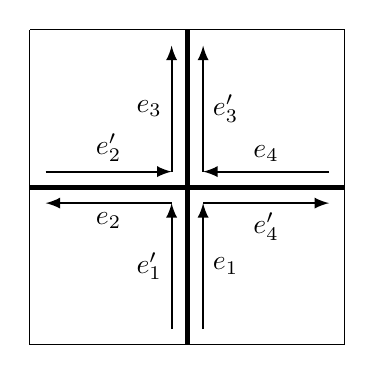
\begin{tikzpicture}
    \coordinate (A0) at (0,0);
    \coordinate (A1) at (2,0);
    \coordinate (A2) at (2,2);
    \coordinate (A3) at (0,2);
    \coordinate (A4) at (4,0);
    \coordinate (A5) at (4,2);
    \coordinate (A6) at (4,4);
    \coordinate (A7) at (2,4);
    \coordinate (A8) at (0,4);
    
    \coordinate (B0) at (0.2,0.2);
    \coordinate (B1) at (1.8,0.2);
    \coordinate (B2) at (1.8,1.8);
    \coordinate (B3) at (0.2,1.8);
    \coordinate (B4) at (2.2,0.2);
    \coordinate (B5) at (3.8,0.2);
    \coordinate (B6) at (3.8,1.8);
    \coordinate (B7) at (2.2,1.8);
    \coordinate (B8) at (0.2,2.2);
    \coordinate (B9) at (1.8,2.2);
    \coordinate (B10) at (1.8,3.8);
    \coordinate (B11) at (0.2,3.8);
    \coordinate (B12) at (2.2,2.2);
    \coordinate (B13) at (3.8,2.2);
    \coordinate (B14) at (3.8,3.8);
    \coordinate (B15) at (2.2,3.8);

     \draw (A0) -- (A1);
     \draw [ultra thick](A1) -- (A2);
     \draw  [ultra thick](A2) -- (A3);
     \draw (A3) -- (A0);
     \draw (A1) -- (A4);
     \draw (A4) -- (A5);
     \draw [ultra thick](A5) -- (A2);
     \draw (A3) -- (A8);
     \draw (A8) -- (A7);
     \draw (A7) -- (A6);
     \draw (A6) -- (A5);
     \draw [ultra thick] (A7) -- (A2);

     \draw [thick,-latex,] (B1) -- (B2);
     \draw [thick,-latex,] (B2) -- (B3);
     \draw [thick,-latex,] (B7) -- (B6);
     \draw [thick,-latex,] (B4) -- (B7);
     \draw [thick,-latex,] (B8) -- (B9);
     \draw [thick,-latex] (B9) -- (B10);
     \draw [thick,-latex,] (B13) -- (B12);
     \draw [thick,-latex,] (B12) -- (B15);
     \node [left] at (1.8, 1) {$e_1'$};
     \node [right] at (2.2, 1) {$e_1$};
     \node [left] at (1.8, 3) {$e_3$};
     \node [right] at (2.2, 3) {$e_3'$};
     \node [below] at (1, 1.8) {$e_2$};
     \node [above] at (1, 2.2) {$e_2'$};
     \node [below] at (3, 1.8) {$e_4'$};
     \node [above] at (3, 2.2) {$e_4$};  \end{tikzpicture}
  \caption{Vertex traversal without boundary and with moibus connection}
  \label{figure:traversalAroundVertexMobius}
\end{figure}
%Figure4
\begin{figure}[ht]
  \centering
  %Normal Junction
  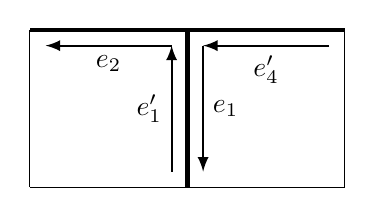
\begin{tikzpicture}
    \coordinate (A0) at (0,0);
    \coordinate (A1) at (2,0);
    \coordinate (A2) at (2,2);
    \coordinate (A3) at (0,2);
    \coordinate (A4) at (4,0);
    \coordinate (A5) at (4,2);
    
    \coordinate (B0) at (0.2,0.2);
    \coordinate (B1) at (1.8,0.2);
    \coordinate (B2) at (1.8,1.8);
    \coordinate (B3) at (0.2,1.8);
    \coordinate (B4) at (2.2,0.2);
    \coordinate (B5) at (3.8,0.2);
    \coordinate (B6) at (3.8,1.8);
    \coordinate (B7) at (2.2,1.8);

     \draw (A0) -- (A1);
     \draw [ultra thick](A1) -- (A2);
     \draw  [ultra thick](A2) -- (A3);
     \draw (A3) -- (A0);
     \draw (A1) -- (A4);
     \draw (A4) -- (A5);
     \draw [ultra thick](A5) -- (A2);

     \draw [thick,-latex,] (B1) -- (B2);
     \draw [thick,-latex,] (B2) -- (B3);
     \draw [thick,-latex,] (B6) -- (B7);
     \draw [thick,-latex,] (B7) -- (B4);
     
     \node [left] at (1.8, 1) {$e_1'$};
     \node [right] at (2.2, 1) {$e_1$};
     \node [below] at (1, 1.8) {$e_2$};
     \node [below] at (3, 1.8) {$e_4'$};
  \end{tikzpicture}
  \caption{Vertex traversal withboundary and without moibus connection}
  \label{figure:traversalAroundVertexNormalB}
\end{figure}

%Figure5
\begin{figure}[ht]
  \centering
  %Normal Junction
  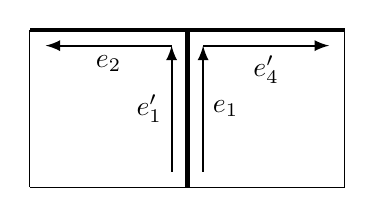
\begin{tikzpicture}
    \coordinate (A0) at (0,0);
    \coordinate (A1) at (2,0);
    \coordinate (A2) at (2,2);
    \coordinate (A3) at (0,2);
    \coordinate (A4) at (4,0);
    \coordinate (A5) at (4,2);
    
    \coordinate (B0) at (0.2,0.2);
    \coordinate (B1) at (1.8,0.2);
    \coordinate (B2) at (1.8,1.8);
    \coordinate (B3) at (0.2,1.8);
    \coordinate (B4) at (2.2,0.2);
    \coordinate (B5) at (3.8,0.2);
    \coordinate (B6) at (3.8,1.8);
    \coordinate (B7) at (2.2,1.8);

     \draw (A0) -- (A1);
     \draw [ultra thick](A1) -- (A2);
     \draw  [ultra thick](A2) -- (A3);
     \draw (A3) -- (A0);
     \draw (A1) -- (A4);
     \draw (A4) -- (A5);
     \draw [ultra thick](A5) -- (A2);

     \draw [thick,-latex,] (B1) -- (B2);
     \draw [thick,-latex,] (B2) -- (B3);
     \draw [thick,-latex,] (B7) -- (B6);
     \draw [thick,-latex,] (B4) -- (B7);
     
     \node [left] at (1.8, 1) {$e_1'$};
     \node [right] at (2.2, 1) {$e_1$};
     \node [below] at (1, 1.8) {$e_2$};
     \node [below] at (3, 1.8) {$e_4'$};

  \end{tikzpicture}
  \caption{Vertex traversal with boundary and with moibus connection}
  \label{figure:traversalAroundVertexMobiusB}
\end{figure}

\newpage

\section{Catumll-Clark Subdivision} \label{sec:ccsd}

Catmull-Clark subdivision is a recursive call on a mesh that we build in section X. Four each level of Catmull-Clark subdivision, we divide every polygon face in the mesh into N quadrilateral faces, where N is the number of halfedges of the polygon face. The new vertices for these sub-faces can be classified into three groups: 1) face points, 2) edge points, and 3) vertex points. We also need to add adjacency information to new sub-faces so that they can be subdivided for the next level. Therefore, each level of subdivision is done in two steps: 1) compute the positions of new vertices, and 2) compile a new mesh given the new vertices.

\subsection{Compute New Vertex Positions}
There are three steps to compute the positions of vertices in the new mesh: 1) make new face points, 2) make new edge points, and 3) make new Vertex Points. Apart from finding the positions for these new vertices, we also need to assign unique IDs for them so no collision will occur for the new mesh.

\subsubsection{Face Points}
Face points are related with faces from the mesh. For every face in the mesh, the position of its face point is defined as the average for positions of all vertices belong to this face. If we label the face point as $f$ and vertices of this face as $v_i$, the equation to calculate face point is,

$$v_f = \frac{v_1 + v_2 + ... + v_n}{n}$$

Therefore, in order to get the face point position, we can do a traversal around a face, find all vertices and get the average of their positions.

This step takes O(E) running time, where E is the number of halfedges in the kth level subdivision mesh.

\subsubsection{Edge Points}
Edge points are related with halfedges from the mesh. In this project, we used the idea from (Reference) and define the sharpness of a halfedge as either infinite sharp or smooth. Depends on the position and sharpness of the edge, we have two ways to calculate the edge point. 

If a halfedge does not lie on the boundary, it has a sibling link or mobius link to anther halfedge. For the halfedges that are not marked as sharp, the position of edge point of a halfedge is the average of its start vertex position, end vertex position, the face point position of the face it belongs to, and the face point position of the face its sibling or mobius sibling belongs to. If we label the edge point as $v_e$, the start and end vertices as $v_1$ and $v_2$, the face point of its face is $v_3$ and the face point of its sibling face is $v_4$, the equation to calculate edge point is,

$$v_e = \frac{v_1 + v_2 + v_3 + v_4}{4}$$

If a halfedge lie on the boundary or it is marked as sharp, the position of the edge point is the average of its start vertex position and end vertex position. If we label the edge point as $v_e$, the start and end vertices as $v_1$ and $v_2$, the equation to calculate edge point is,

$$v_e = \frac{v_1 + v_2}{2}$$

This step takes O(E) running time, where E is the number of halfedges in the kth level subdivision mesh.

\subsubsection{Vertex Points}
Vertex points are related with vertices from the mesh. In order to find the vertex point, we traverse around an original vertex in the mesh, find the information we need from adjacent faces and halfedges and count the number of sharp halfedges we cross in the traversal. The number of sharp halfedges linking with this vertex determines methods to calculate vertex points.

1) A vertex with three or more incident sharp edges is called a corner, the new vertex point has same position with the original vertex. If we label the vertex point as $v_p$, the original vertex as $v_1$, the equation to calculate vertex point is,

$$v_p = v_1$$

2) A vertex with two incident sharp edges is called a crease vertex. If we label the vertex point as $v_p$, the original vertex as $v_1$ and the two halfedges are labeled with $v_1v_2$ and $v_1v_3$. The equation to calculate vertex point is,

$$v_p=\frac{v_2 + 6v_1 + v_3}{8}$$

3) A vertex with less than two sharp edges is a normal vertex. There are two different approaches in calculating the vertex point for a normal vertex. We label the vertex point as $v_p$, the original vertex point as $v_1$, the average for all midpoints of edges that contains the original vertex is $v_2$, the average for all edge points of edges that contains the original vertex is $v_2'$, the average of the face points of all faces adjacent to the old vertex point as $v_3$, and the number of faces adjacent to the vertex as $n$, and the number of edges adjacent as $n'$. Catmull-Clark (Reference) defined vertex point as 

$$v_p=\frac{(n - 3)v_1 + 2v_2 + v_3}{n}$$

While DeRose (Reference) defined vertex point as

$$v_p=\frac{(n' - 2)v_1 + v_2' + v_3}{n'}$$

Catmull-Clark's equation used the average of all midpoints of incident edges and has one more weight on it and one less weight on the original vertex. DeRose's equation used the average of all edge points incident to the vertex. Meanwhile, in a mesh with boundary, $n$ and $n'$ would be different by 1. However, the actual difference between these two equations is very small. 

In the example of Figure \ref{figure:differenceCandD}, if we do one more level of calculation and represent the new vertex point only with the original vertices, the results from Catmull-Clark and DeRose equations are,

$$v_p=\frac{18}{32}v_0 + \frac{6}{64}(v_2 + v_4 + v_5 + v_7) + \frac{2}{128}(v_1 + v_3 + v_6 + v_8)$$

and,

$$v_p=\frac{27}{32}v_0 + \frac{3}{64}(v_2 + v_4 + v_5 + v_7) + \frac{3}{128}(v_1 + v_3 + v_6 + v_8)$$

respectively. We can see that Catmull-Clark has more weights on the immediate neighbor vertices $v_2$, $v_4$, $v_5$, and $v_7$, while DeRose has much more on the original vertex. In this project, we used DeRose's equation to calculate vertex point for a normal vertex.

This step takes O(E) running time, where E is the number of halfedges in the kth level subdivision mesh.

\begin{figure}[ht]
  \centering
  \begin{tikzpicture}
    \coordinate (A0) at (0,0);
    \coordinate (A1) at (2,0);
    \coordinate (A2) at (2,2);
    \coordinate (A3) at (0,2);
    \coordinate (A4) at (4,0);
    \coordinate (A5) at (4,2);
    \coordinate (A6) at (4,4);
    \coordinate (A7) at (2,4);
    \coordinate (A8) at (0,4);

    \draw (A0) -- (A1);
    \draw (A1) -- (A2);
    \draw (A2) -- (A3);
    \draw (A3) -- (A0);
    \draw (A1) -- (A4);
    \draw (A4) -- (A5);
    \draw (A5) -- (A2);
    \draw (A3) -- (A8);
    \draw (A8) -- (A7);
    \draw (A7) -- (A6);
    \draw (A6) -- (A5);
    \draw (A7) -- (A2);
    \node [left] at (0, 2) {$v_2$};
    \node [right] at (4, 2) {$v_7$};
    \node [above left] at (0, 4) {$v_1$};
    \node [above right] at (4, 4) {$v_6$};
    \node [below left] at (0, 0) {$v_3$};
    \node [above] at (2, 4) {$v_4$};
    \node [below] at (2, 0) {$v_5$};
    \node [above right] at (2, 2) {$v_0$};
    \node [below right] at (4, 0) {$v_8$};
  \end{tikzpicture}
  \caption{Example of difference of Catmull-Clark and DeRose Equation}
  \label{figure:differenceCandD}
\end{figure}

\subsection{Compile a New Mesh}
The newly generated vertices also need to be linked with each other. We compile the new mesh with traversal around face for every face from the original mesh.

For every halfedge $v_iv_j$ in the face, we create four new halfedges. If we denote its edge point of the current halfedge as $v_e$ and the face point of its face as $v_f$, the four new halfedges are $v_iv_e$, $v_ev_j$, $v_ev_f$, and $v_fv_e$. An example in shown in Figure \ref{figure:compileNewMesh}. The halfedge $v_1v_2$ generated $v_1v_e$, $v_ev_2$, $v_ev_f$, $v_fv_e$. We also add the following adjacency information while generating sub-halfedges: 

1) Add one outgoing halfedge pointer to every new vertex. If the new halfedge is on mobius connection, mark the new vertex on mobius connection.

2) Add previous and next pointers to the sub-halfedges. 

3) Add sibling pointers to every pair of $v_ev_f$ and $v_fv_e$.

4) $v_iv_e$ and $v_ev_j$ need to inherit the sharpness and boundary feature from their parent halfedge, 

5) If $v_iv_j$ is not on boundary, we add sibling links between $v_iv_e$ and the corresponding sub-halfedge of its parent's sibling and add sibling links between $v_ev_j$ and the corresponding sub-halfedge of its parent's sibling.

6) If $v_iv_j$ is on the boundary and has boundary links with its boundary neighbor halfedges, we add boundary links for $v_iv_e$ and the corresponding sub-halfedge of its parent's boundary neighbor. We also add boundary links for $v_iv_e$ and the corresponding sub-halfedge of its parent's boundary neighbor.

\begin{figure}[ht]
  \centering
  \begin{tikzpicture}
    \coordinate (A0) at (0,0);
    \coordinate (A1) at (2,0);
    \coordinate (A2) at (2,2);
    \coordinate (A21) at (2, 2.05);
    \coordinate (A22) at (2, 1.95);
    \coordinate (A3) at (0,2);
    \coordinate (A4) at (4,0);
    \coordinate (A5) at (4,2);
    \coordinate (A51) at (4, 2.05);
    \coordinate (A52) at (4, 1.95);
    \coordinate (A6) at (4,4);
    \coordinate (A7) at (2,4);
    \coordinate (A8) at (0,4);

    \draw (A0) -- (A4);
    \draw [thick, -latex](A4) -- (A5);
    \draw [thick, -latex](A5) -- (A6);
    \draw [thick, -latex](A52) -- (A22);
    \draw [thick, -latex](A21) -- (A51);    
    \draw (A6) -- (A8);
    \draw (A8) -- (A0);
    \node [right] at (4, 0) {$v_1$};
    \node [above left] at (0, 4) {$v_3$};
    \node [above right] at (4, 4) {$v_2$};
    \node [below left] at (0, 0) {$v_0$};
    \node [above right] at (2, 2) {$v_f$};
    \node [below right] at (4, 2) {$v_e$};
  \end{tikzpicture}
  \caption{Create four sub-halfedges for one halfedge in subdivision.}
  \label{figure:compileNewMesh}
\end{figure}

When the traversal around face is done for every face in the level k subdivision mesh, the level k + 1 subdivision mesh would be created.

This step takes O(E') running time, where E' is the number of halfedges in the (k + 1)th level subdivision mesh.

As a summary, the Catmull-Clark at kth level takes O(E') running time, where E' is the number of halfedges in the (k + 1)th level subdivision mesh.

\newpage
\section{Offset Mesh} \label{sec:offset}

The offset with value offVal for a mesh M contains three parts: 1) Positive offset, where we translate every vertex of M by offVal along the direction of its vertex normal, 2) Negative offset, where we translate every vertex of M by offVal along the opposite direction of its vertex normal, and 3) the cover mesh between positive offset and negative offset, which is the extrusion for M's boundaries along positive and negative vertex normal direction. This offset mesh is a two-sided surface with no mobius connections.

In two-sided surfaces, the positive offset mesh is always separated from the negative mesh. However, in single-sided surfaces, the positive offset mesh will be connected with the negative mesh at the mobius connection of the original mesh.

In order to get the offset mesh, we need two steps: 1) calculate vertex normal for all vertices from the original mesh, 2) build positive and negative offset meshes, and 3) build cover mesh between positive and negative offsets.

\subsection{Compute Vertex Normal}
The vertex normal for a vertex is commonly defined as the average for the surface normal of all faces adjacent to the vertex. To get the surface normal for a face of N polygon, we use Newell's Method.

\subsubsection{Newell's Method and Surface Normal}
Newell's method defines the surface normal as the normalized average for cross products of all consecutive halfedges in the face. For a polygon face with n halfedges, we denote them as $v_0v_1$, $v_1v_2$, ...,$v_{n-1}v_0$, where $ n \ge 3$. The surface normal $N_{f}$ is,

$$N_{f} = normalize(\sum\limits_{i=1}^{n-2} (v_i - v_{i - 1}) \times (v_{i + 1} - v_{i}) + (v_{n - 1} - v_{n - 2}) \times (v_0 - v_{n - 1}) + (v_0 - v_{n - 1}) \times (v_1 - v_0))$$

Therefore, we calculate surface normal for every face in the mesh by traversal around face. It takes O(E) running time, where E is the number of halfedges in the mesh.

\subsubsection{Vertex normal}
We calculate vertex normal by traversal around vertex. If a vertex $v$ is not on a mobius connction, we denote the m faces adjacent to vertex $v$ are $f_0, f_1, ..., f_m$, the vertex normal $N_v$ is,

$$N_{v} = normalize(\sum\limits_{i=1}^{m-1} N_{f_i})$$

However, when $v$ is on mobius connection, the halfedge flows for some adjacent faces are in opposite directions (clockwise vs. counter clockwise). It leads to surface normal in opposite directions. We need to fix this issue by introducing a mobius counter. In the vertex traversal, we start by adding the surfaces normal when we find a face. When we cross a mobius connection, we add the negative surface normal for the upcoming faces until we cross another mobius connection.

Another way to address this mobius vertex issue is to check the dot product of every surface normal with the sum that we have got. If the dot product is positive, we add this surface normal, if not, we add its negative surface normal.

Calculating all vertex normal takes O(E) running time, where E is the number of halfedges in the mesh.

\subsection{Positive and Negative Offset Meshes}

For a mesh with no mobius connection, the positive and negative offset meshes will have no connection with each other. We get the positive offset by copy the mesh, and translate every vertex along its normal with an offset value. 

For negative offset, we still want to copy the mesh but the halfedge flow in the faces is in opposite directions. We then translate every vertex along the opposite direction of its normal with an offset value.

When there is a mobius connection, positive offset mesh and negative offset will join each other at the mobius connection. Normal of vertices on mobius connection may not reflect the direction for its positive translation. 

In this project, we make the translations of vertex positions with traversal around face. If a vertex is on mobius connection, we can check the dot product of its normal and the face normal for the face it belongs to. If the dot product is positive, we translate along this vertex normal for its positive offset and the opposite for its negative offset. If the dot product is negative, we translate along this vertex normal for its negative offset and the opposite for its positive offset.

This step takes O(E) running time, where E is the number of halfedges in the mesh.

\subsection{Cover Mesh}

We also need to build the cover mesh to connect positive offset with negative offset. For a mesh with no mobius connection, we traverse along its boundary. For every halfedge $v_iv_j$ on the boundary, we build a quadrilateral face $v_{posJ}v_{posI}v_{negI}v_{negJ}$, where $v_{posI}$ and $v_{posJ}$ are the positive offset for $v_i$ and $v_j$, and $v_{negI}$ and $v_{negJ}$ are the negative offset for $v_i$ and $v_j$.

As we mentioned before, normal of vertices on mobius connection may not reflect the direction for its positive translation. For a vertex $v_i$ on mobius connection, we need to check the dot product of its normal with the surface normal that it belongs to. If the dot product is positive, we use $v_i$'s vertex normal to calculate $v_{posI}$ and negative vertex normal to calculate $v_{negI}$. If the dot product is negative, we use $v_i$'s vertex normal to calculate $v_{negI}$ and negative vertex normal to calculate $v_{posI}$. After this check for $v_i$ and $v_j$, we build the quadrilateral face $v_{posJ}v_{posI}v_{negI}v_{negJ}$.

This step takes O(E) running time, where E is the number of boundary halfedges in the mesh.

The offset mesh will be the combination of the positive offset, negative offset and cover mesh that we build above. In total, it takes O(E) running time to build the offset mesh.

\subsection{Offset vs. Subdivision}
A question was raised on whether we do offset first or subdivision first. The answer depends on our expectation for the sharpness between the cover mesh and positive/negative offset mesh of the final product. If we want a smooth curve, then offset should be done first. If we want it as a sharp edge, then subdivision should be done first. A combination of pre-subdivision, post-subdivision and offset (e.g. 2 levels of subdivision, offset, another 2 levels of subdivision) can lead to a smooth curve between the two above.

If we do offset first, the initial mesh for subdivision will be a two-sided surface with no mobius connection. The down side of doing offset first, however, is that we have more than twice of amount of elements in the offset mesh. It will take double running time to get the final result.

\newpage
\section{Input and Output}
The input and output of subdivision or offset are polygon meshes. Figure \ref{figure:birdView} gives a broader view of this subdivision/offset machine. We need to produce the initial mesh for subdivision and display its output mesh in certain ways.

\tikzstyle{block} = [rectangle, draw, 
    text width=6.5em, text centered, rounded corners, minimum height=1em]
\tikzstyle{line} = [draw, -latex']

\begin{figure}[ht]
  \centering    
  \begin{tikzpicture}[node distance = 3.5cm, auto]
      % Place nodes
      \node [block] (GUIINPUT) {GUI INPUT};
      \node [block, below right of=GUIINPUT] (INITMESH) {INITIAL MESH};
      \node [block, below left of=INITMESH] (FILEINPUT) {FILE INPUT};
      \node [block, right of=INITMESH] (SDOFF) {SUBDIVISION MACHINE};
      \node [block, right of=SDOFF] (NEWMESH) {NEW MESH};
      \node [block, above right of=NEWMESH] (GUIOUTPUT) {GUI OUTPUT};
      \node [block, below right of=NEWMESH] (FILEOUTPUT) {FILE OUTPUT};
      % Draw edges
      \path [line] (GUIINPUT) -- (INITMESH);
      \path [line] (FILEINPUT) -- (INITMESH);
      \path [line] (INITMESH) -- (SDOFF);
      \path [line] (SDOFF) -- (NEWMESH);
      \path [line] (NEWMESH) -- (GUIOUTPUT);
      \path [line] (NEWMESH) -- (FILEOUTPUT);
  \end{tikzpicture}
    \caption{A broader view of the subdivision machine}
    \label{figure:birdView}
\end{figure}

\subsection{Input}
The basic information we need to build an initial mesh is: 1) the position for all vertices in the mesh, and 2) the polygon defined with these vertices.
This information can be retrieved in two ways. It can come from the graphical user interface. Or it is read from a file contains vertex and polygon information.
\subsubsection{Input File Parser}
Currently, the input of initial polygon mesh comes from file input, which defines the position of vertices, and how polygons are built from these vertices. As long as the polygons are defined in a continuous flow of halfedges, or a loop of consecutive vertices in the right order, it is good to build the initial mesh of subdivision.

A question was raised on the read of vertices. As mentioned in section X, the assumption of vertex in the mesh is ``no two vertices share same position in a mesh". The problem of vertex having same positions is that mesh at that position is seen as a boundary.  The subdivision will shrink the mesh at this boundary and so it will be separated. Here, we define ``same position" as the distance between two vertex is smaller than a tolerance value.

Reading from the input file, if the parser finds a new vertex having same position that we parsed before, we can merge these two vertices immediately. Or we can keep both of them as different vertices and create a temporary mesh. We then go through the boundary of the temporary mesh and check if any two halfedges can be merged. The problem with merging immediately is that the merge operation should be done on the unit of halfedge in order to maintain the property of 2-manifold. 

If we force to merge vertex immediately, it may result in a non-2-manifold geometry. In the example of Figure \ref{figure:parserMerge}, $v_0$ and $v_0'$ are very close to each other (probably smaller than the tolerance we defined). If we merge these two vertices directly, the result will be a non-2-manifold and the program can not figure out how to trace the boundary of this geometry.

\begin{figure}[ht]
  \centering
  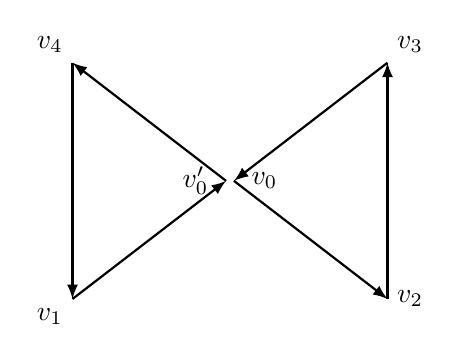
\begin{tikzpicture}
    \coordinate (A0) at (0,0);
    \coordinate (A1) at (2,0);
    \coordinate (A2) at (2,1.5);
    \coordinate (A21) at (2.05, 1.5);
    \coordinate (A22) at (1.95, 1.5);
    \coordinate (A3) at (0,1.5);
    \coordinate (A4) at (4,0);
    \coordinate (A5) at (4,1.5);
    \coordinate (A51) at (4, 1.45);
    \coordinate (A52) at (4, 1.55);
    \coordinate (A6) at (4,3);
    \coordinate (A7) at (2,3);
    \coordinate (A8) at (0,3);

    \draw [thick, -latex](A0) -- (A22);
    \draw [thick, -latex](A22) -- (A8);
    \draw [thick, -latex](A8) -- (A0);
    \draw [thick, -latex](A4) -- (A6);
    \draw [thick, -latex](A6) -- (A21);
    \draw [thick, -latex](A21) -- (A4);

    \node [right] at (4, 0) {$v_2$};
    \node [above left] at (0, 3) {$v_4$};
    \node [above right] at (4, 3) {$v_3$};
    \node [below left] at (0, 0) {$v_1$};
    \node [right] at (2.15, 1.5) {$v_0$};
    \node [left] at (1.85, 1.5) {$v_0'$};

  \end{tikzpicture}
  \caption{Problem of merging vertex immediately when parsing the file.}
  \label{figure:parserMerge}
\end{figure}

Another issue of parsing is associated with the extraordinary points in Catmull-Clark subdivision. Polygons that are not quadrilaterals will generate extraordinary points in the mesh. We preferably want as less extraordinary points as possible. Therefore, when parsing files with triangle definitions, it is a good practice to combine two triangles that share an edge into a quadrilateral.

\subsubsection{Graphical User Interface}
In a graphical user interface (GUI), a user can 1) draw the points in 3D space, 2) link these vertices into polygons, and 3) tell the program to merge the boundary of two meshes. 

In order to do 1), the user can click and select point on screen, or use points on a bezier curve or bspline. To do 2), the user select points consecutively and ends up a loop. In the future, we want the user can do 1) and 2) simultaneously by creating a higher order geometry, like a funnel, tunnel, sweep lines, bezier curve or bsplines.

\subsection{Output}
\subsubsection{Graphical User Interface}
In this project, we display the output of the subdivision machine in OpenGL and GLUT (The OpenGL utility toolkit). 
Arcball feature is applied so the user can rotate the mesh with mouse control and view it from different directions. 
Keyboard controls are also applied so the user can 1) zoom in and out, 2) switch between flat shading and smooth shading, and 3) switch between the polygon mode and wireframe mode.
\subsubsection{Output Files}
In this project the output mesh can also be saved and written to a geometry definition file. For example, the STL file produced by this program can be displayed by other viewers, such as 3D Builder from Microsoft or the online viewer of github. It can also be passed to prototype software like QuickSlice and be 3D printed.

\newpage
\section{Test Cases}
Two test cases were given to this subdivision machine to test the result of Catmull-Clark subdivision. The initial meshes for these test cases were the work of Professor Carlos Sequin. (The figures are now at the end of this report.)
\subsection{Hild Sculpture}
Hild Sculpture is a two-sided geometry. The initial mesh is shown in Figure \ref{figure:Hild0}, level 1, level 2, and level 3 subdivisions are shown in Figure \ref{figure:Hild1} to \ref{figure:Hild3}. Offset after 2 level of subdivision is shown in Figure \ref{figure:HildOff}.

\begin{figure}[h!]
  \centering
    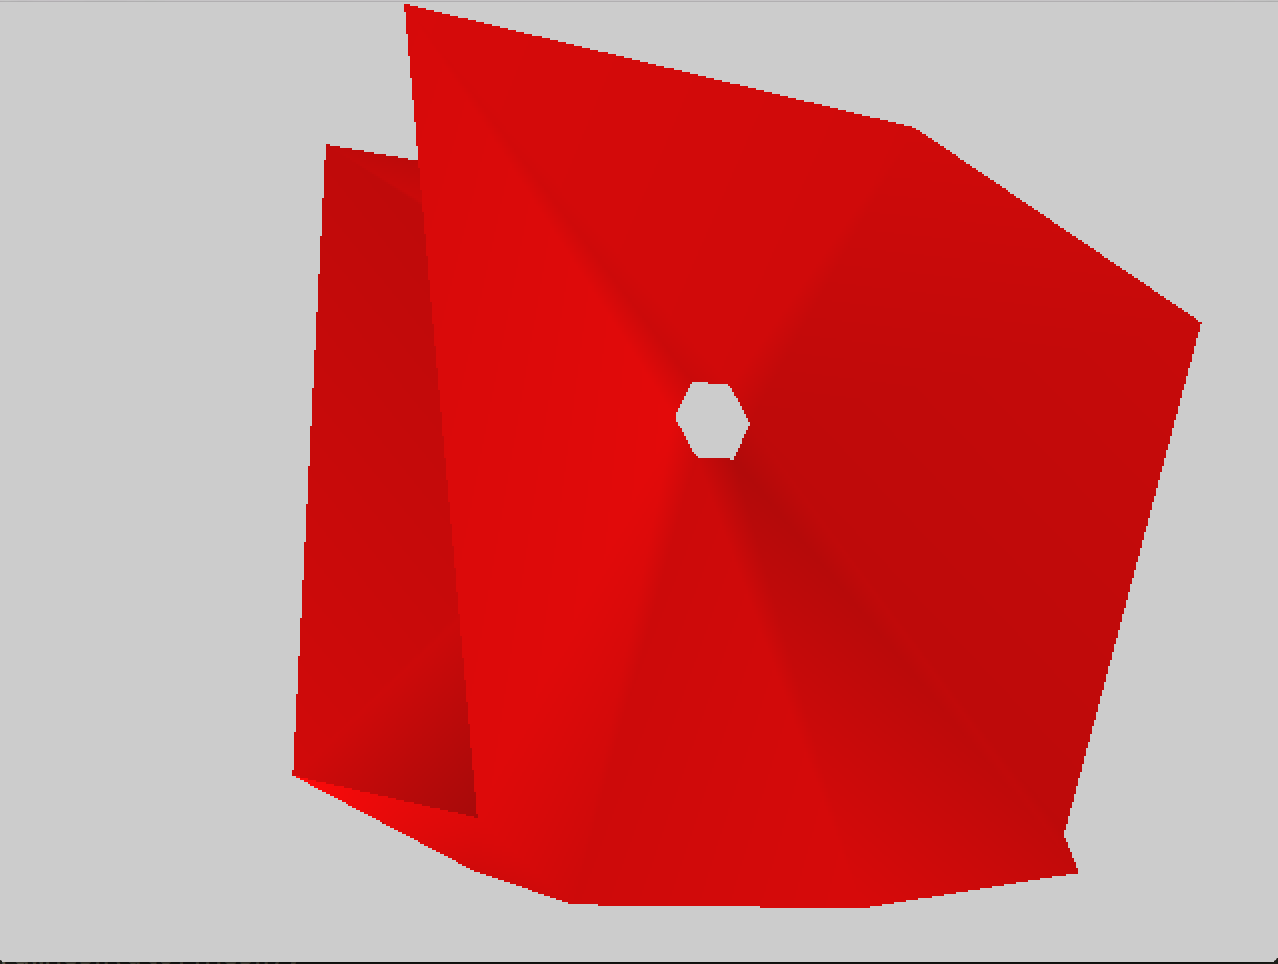
\includegraphics[width=\textwidth]{Hild0}
    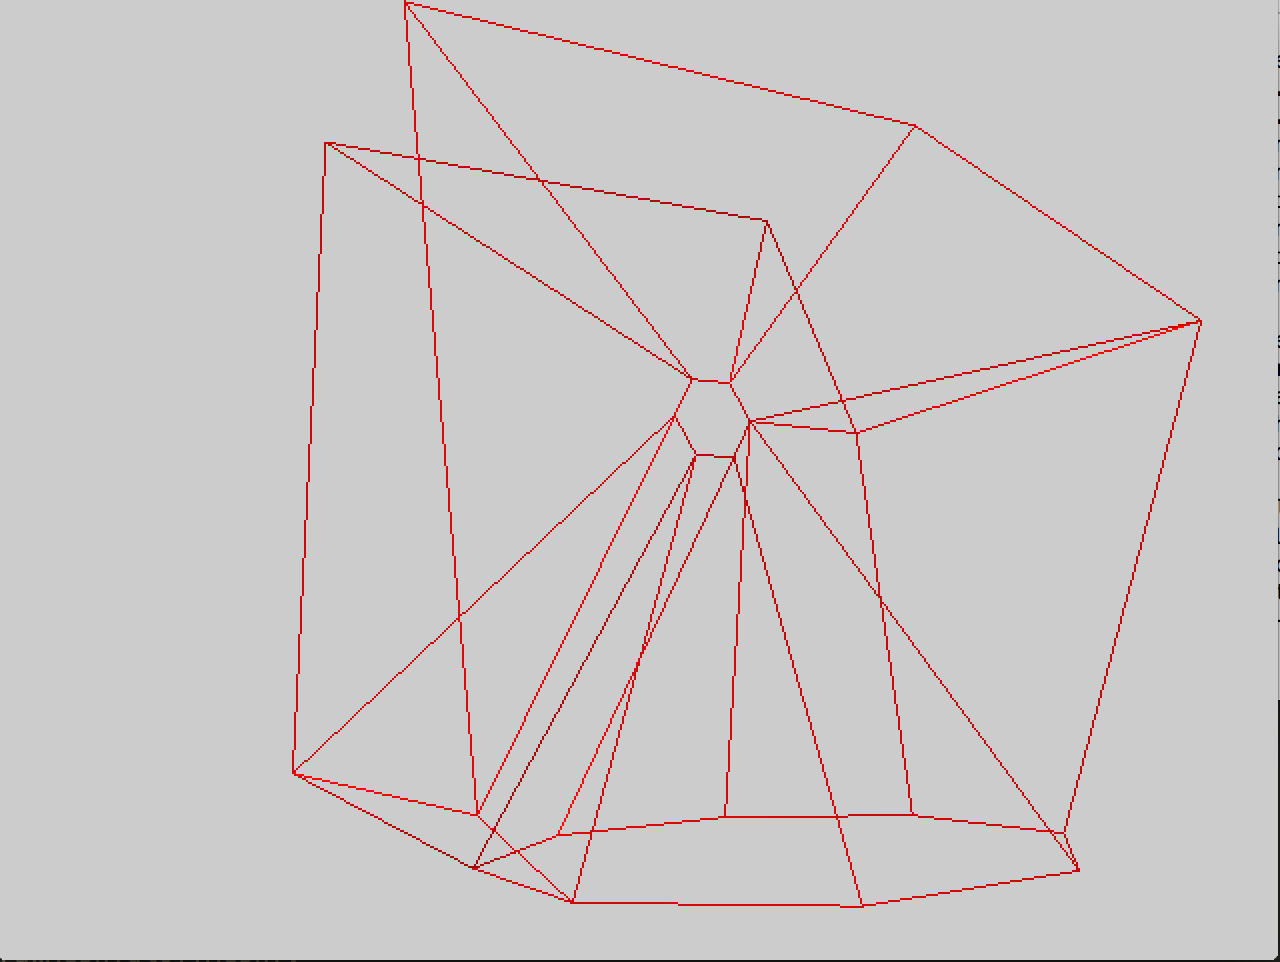
\includegraphics[width=\textwidth]{Hild0w}
  \caption{Initial Mesh of Hild Sculpture.} \label{figure:Hild0}
\end{figure}

\begin{figure}[h!]
  \centering
    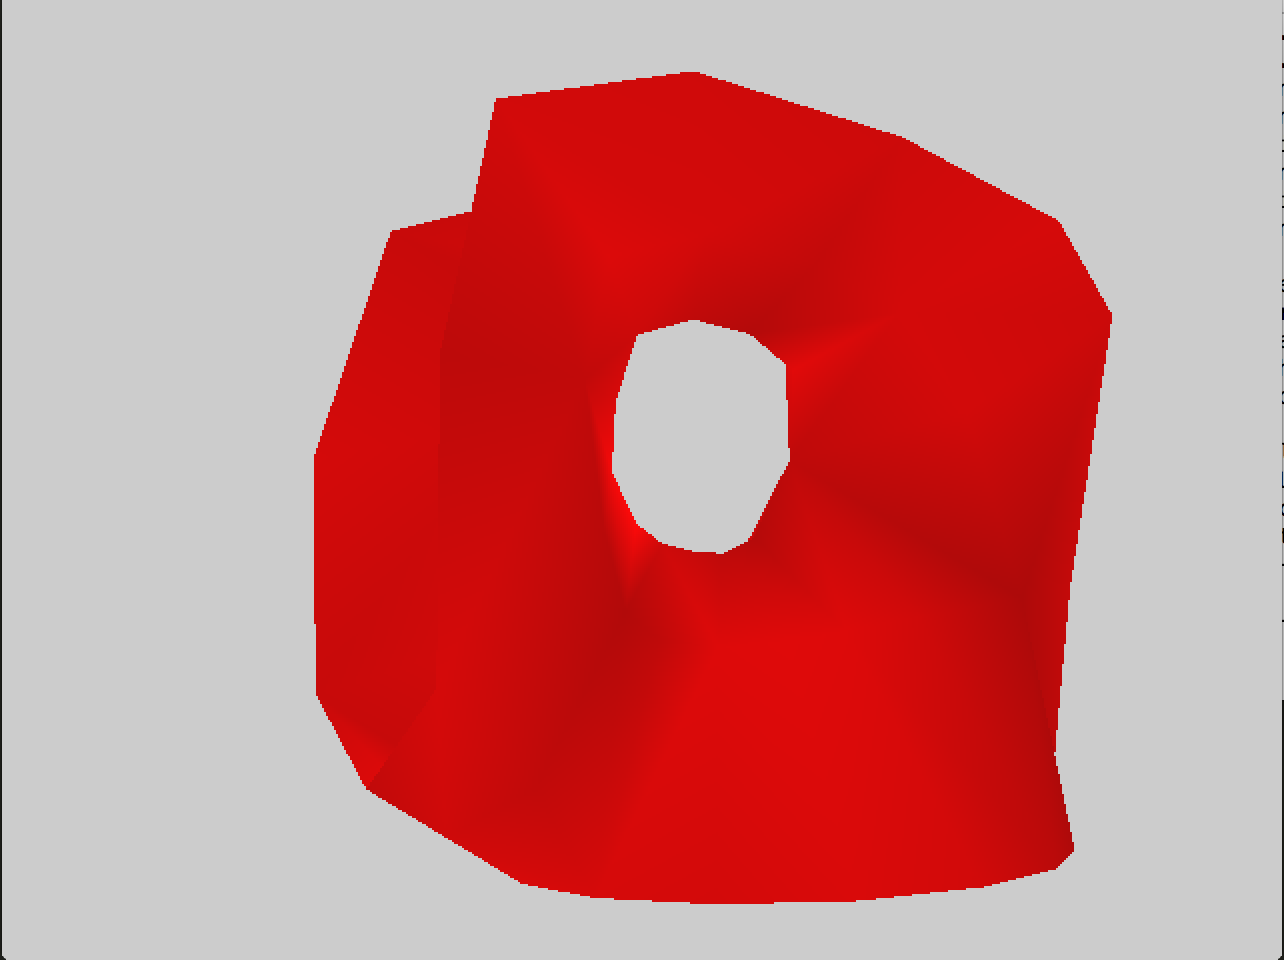
\includegraphics[width=\textwidth]{Hild1}
    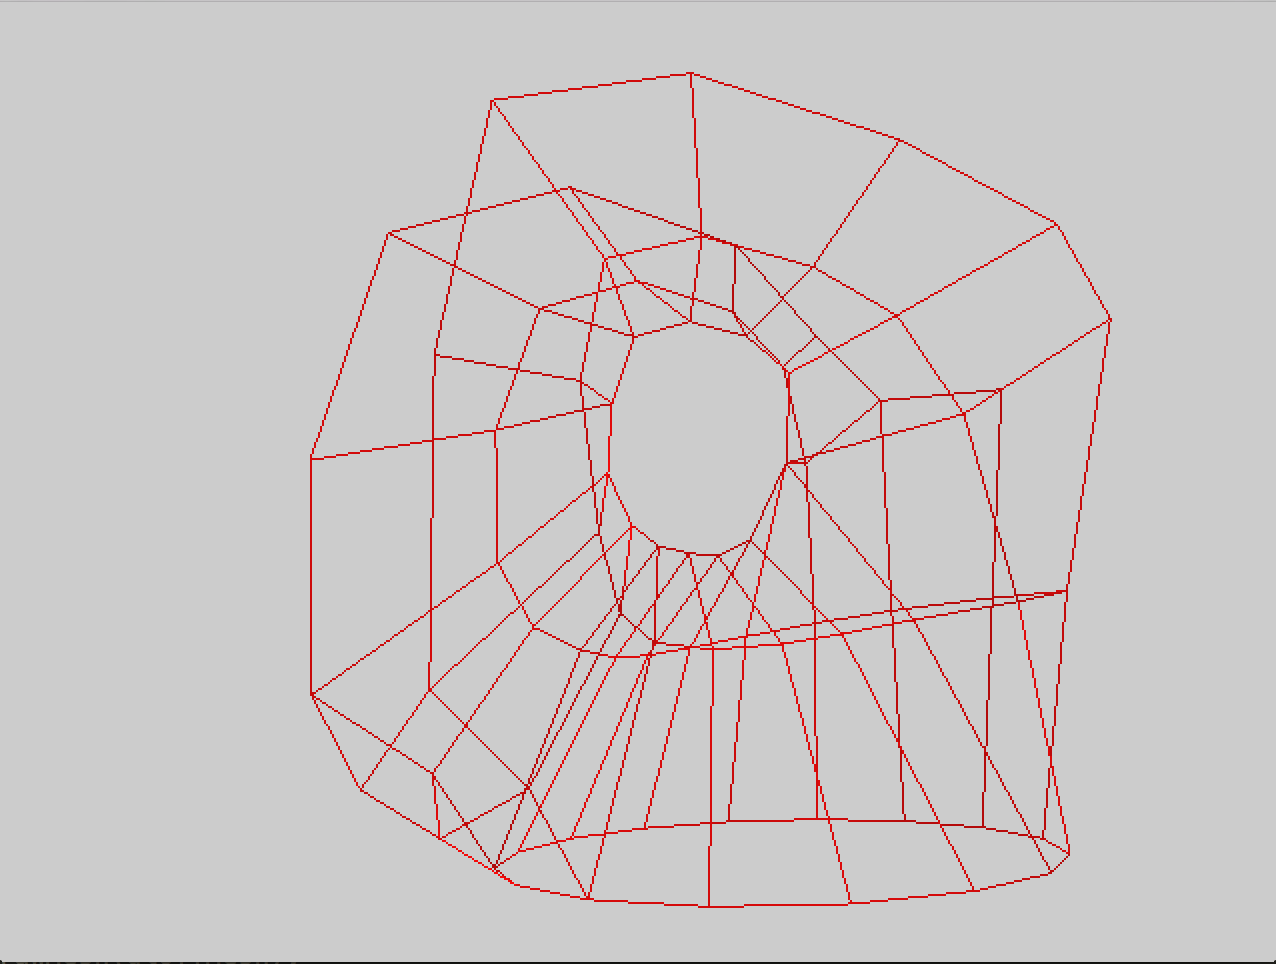
\includegraphics[width=\textwidth]{Hild1w}
  \caption{1 Level Subdivision of Hild Sculpture.} \label{figure:Hild1}
\end{figure}

\begin{figure}[h!]
  \centering
    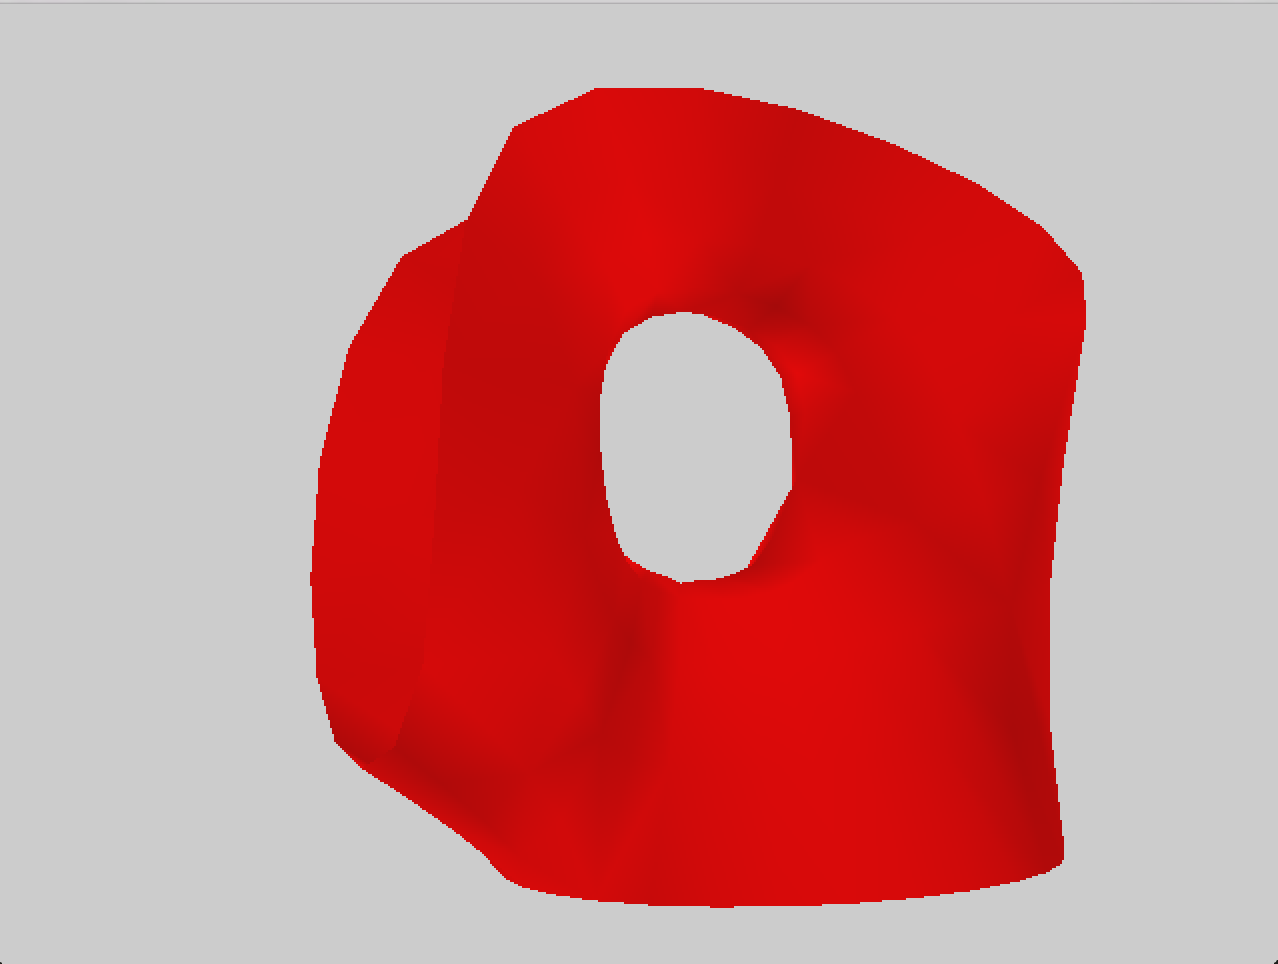
\includegraphics[width=\textwidth]{Hild2}
    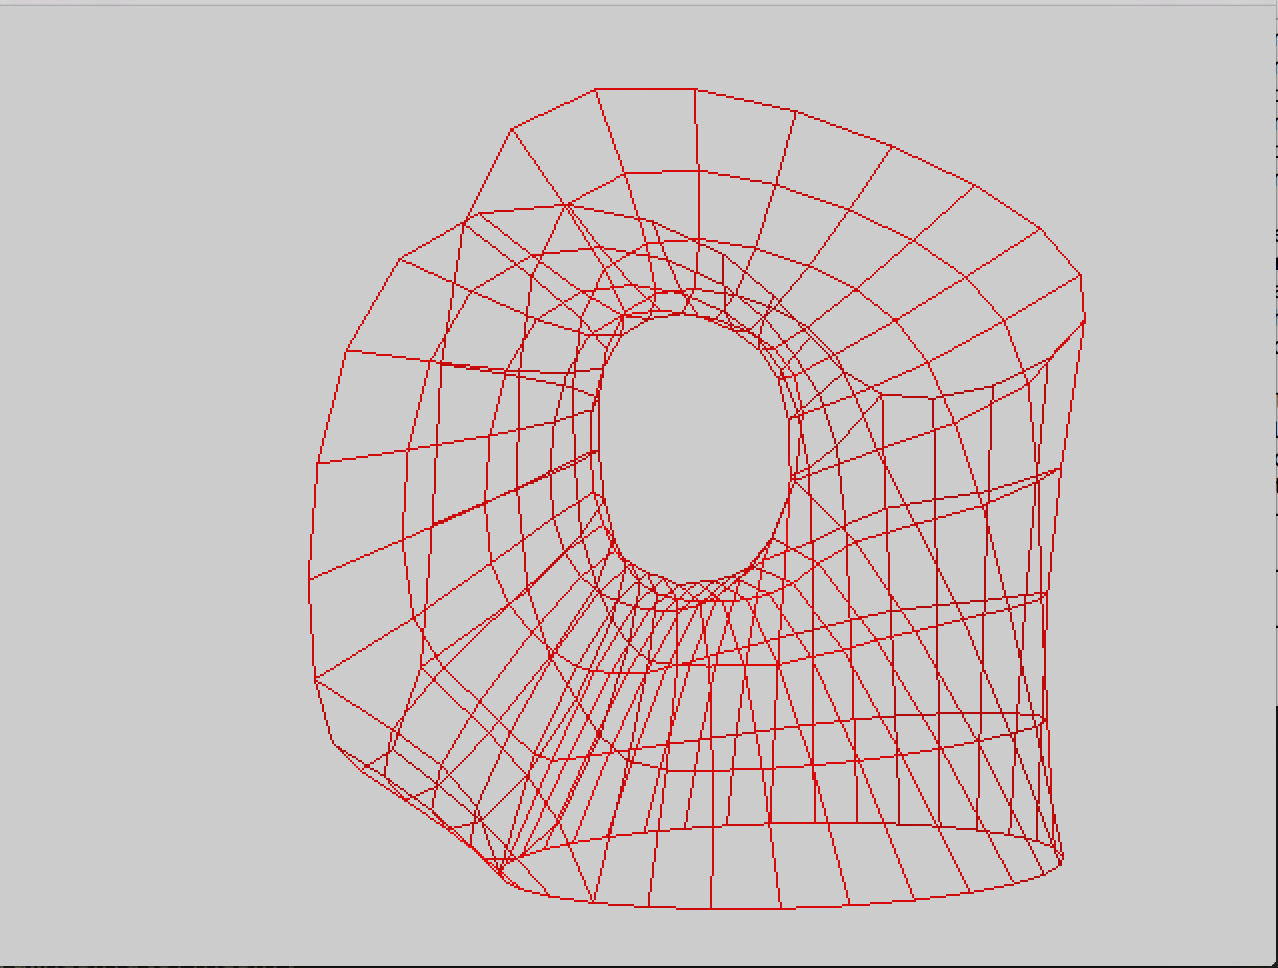
\includegraphics[width=\textwidth]{Hild2w}
  \caption{2 Levels Subdivision of Hild Sculpture.} \label{figure:Hild2}
\end{figure}

\begin{figure}[h!]
  \centering
    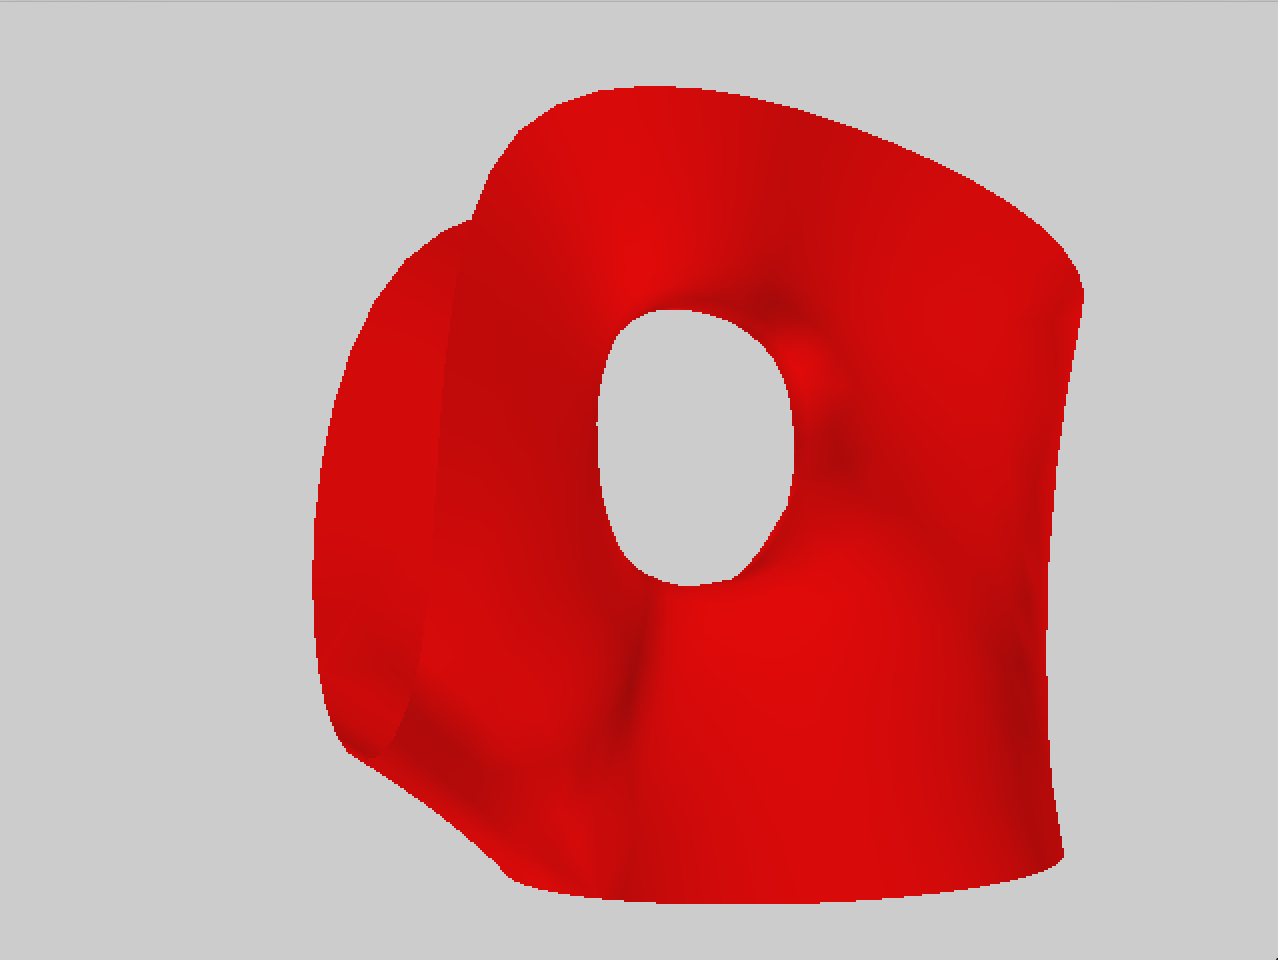
\includegraphics[width=\textwidth]{Hild3}
    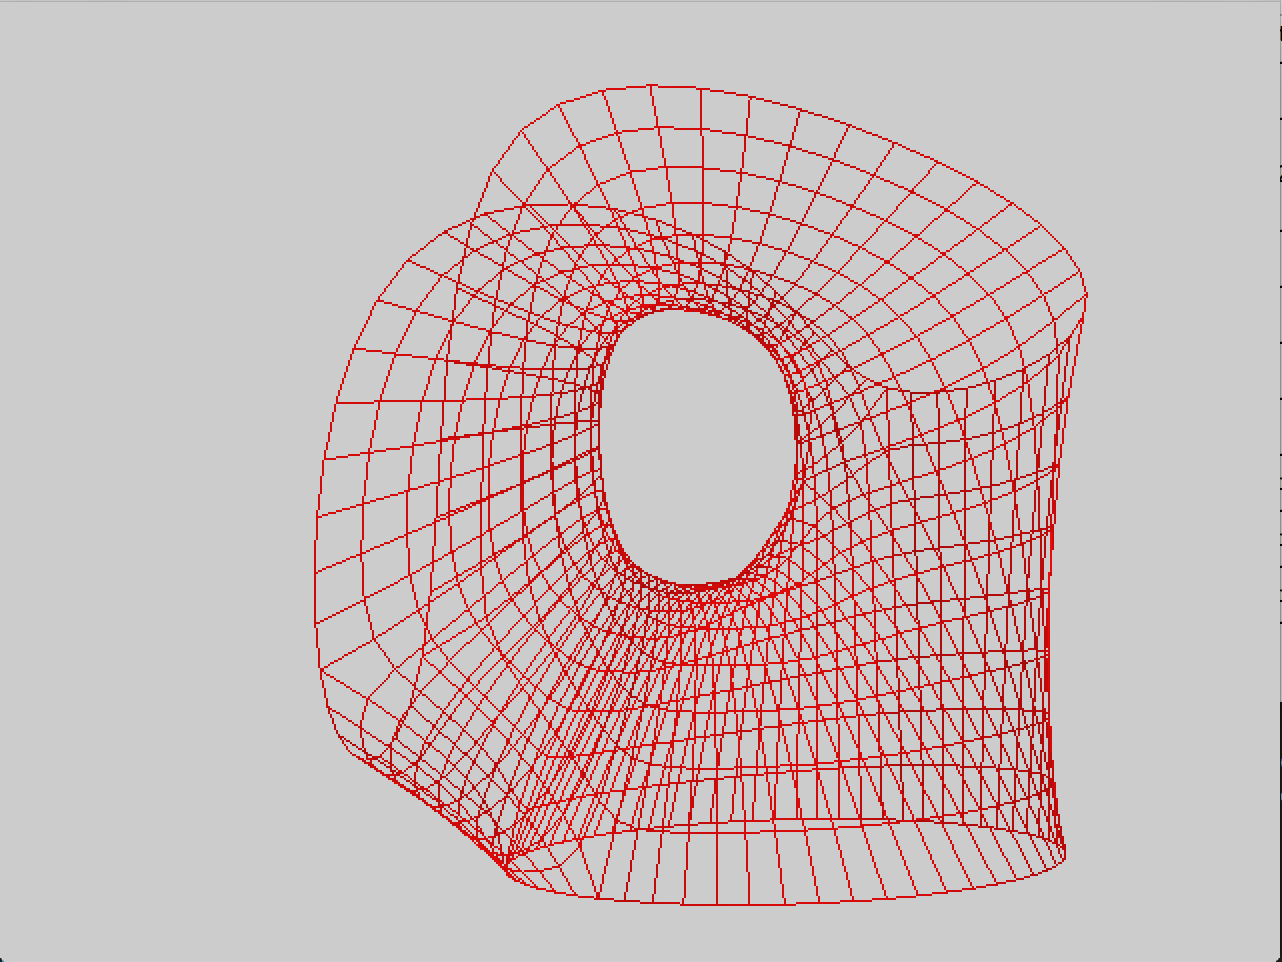
\includegraphics[width=\textwidth]{Hild3w}
  \caption{3 Levels of Subdivision of Hild Sculpture.} \label{figure:Hild3}
\end{figure}

\begin{figure}[h!]
  \centering
    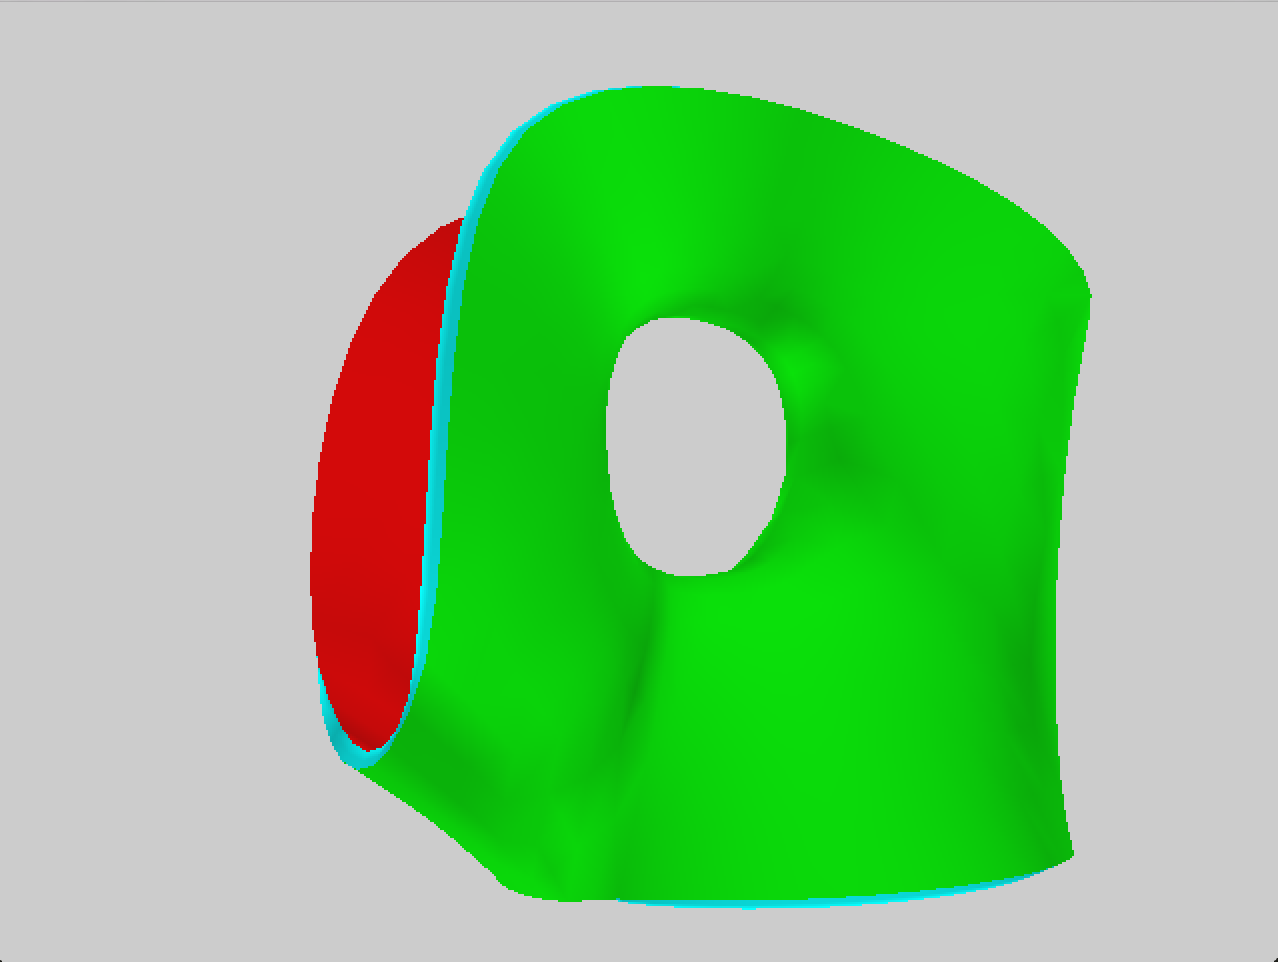
\includegraphics[width=\textwidth]{HildOff}
  \caption{Offset after 3 Levels of Subdivision of Hild Sculpture.} \label{figure:HildOff}
\end{figure}

\subsection{Tetra Sculpture}
Tetra is a single-sided geometry with 4 mobius connections. The initial mesh is shown in Figure \ref{figure:Tetra0}, level 1, level 2, and level 3 subdivisions are shown in Figure \ref{figure:Tetra1} to \ref{figure:Tetra3}. Offset after 2 level of subdivision is shown in Figure \ref{figure:TetraOff}.

\begin{figure}[h!]
  \centering
    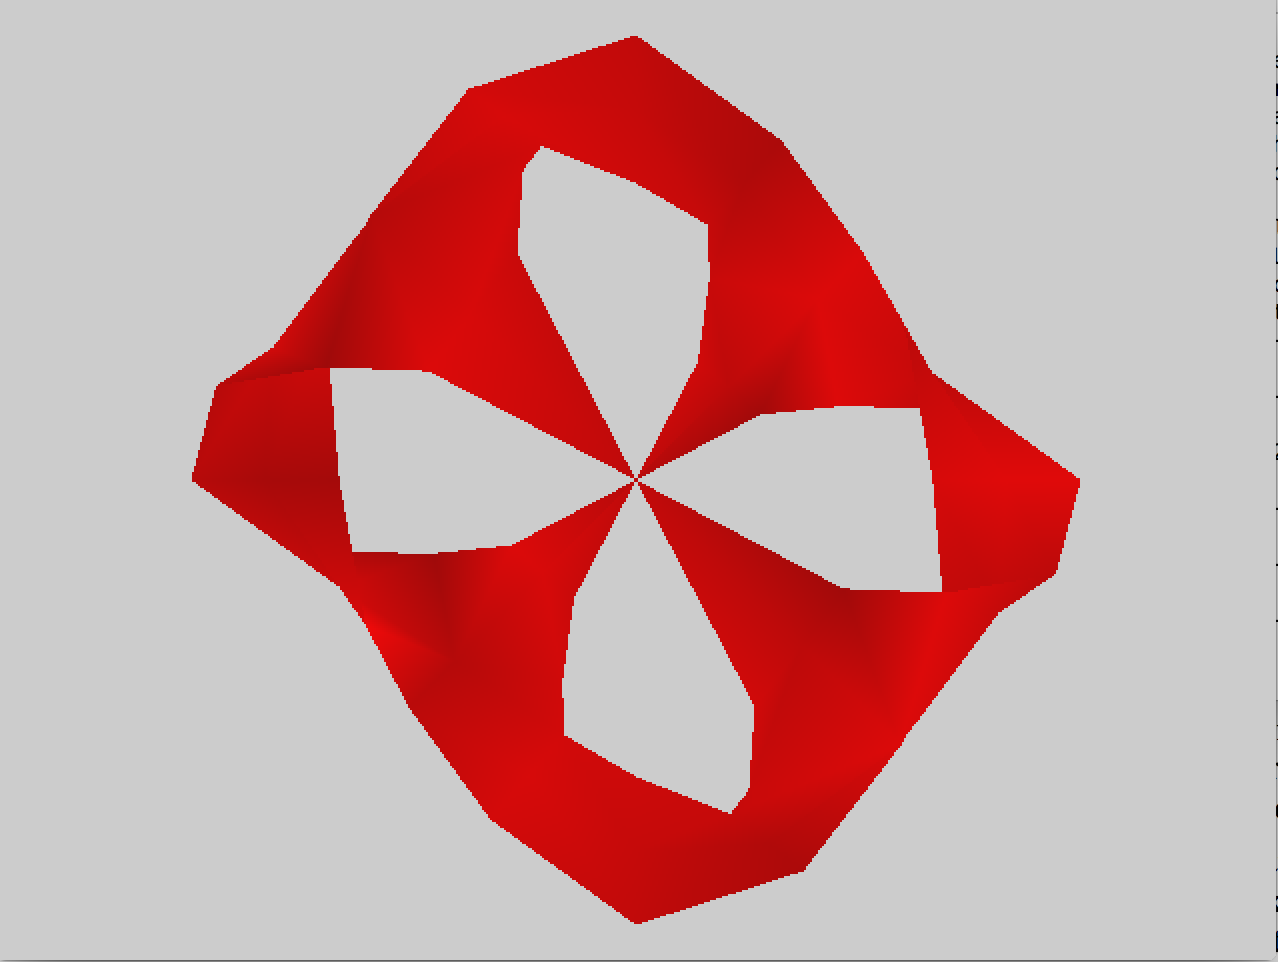
\includegraphics[width=\textwidth]{Tetra0}
    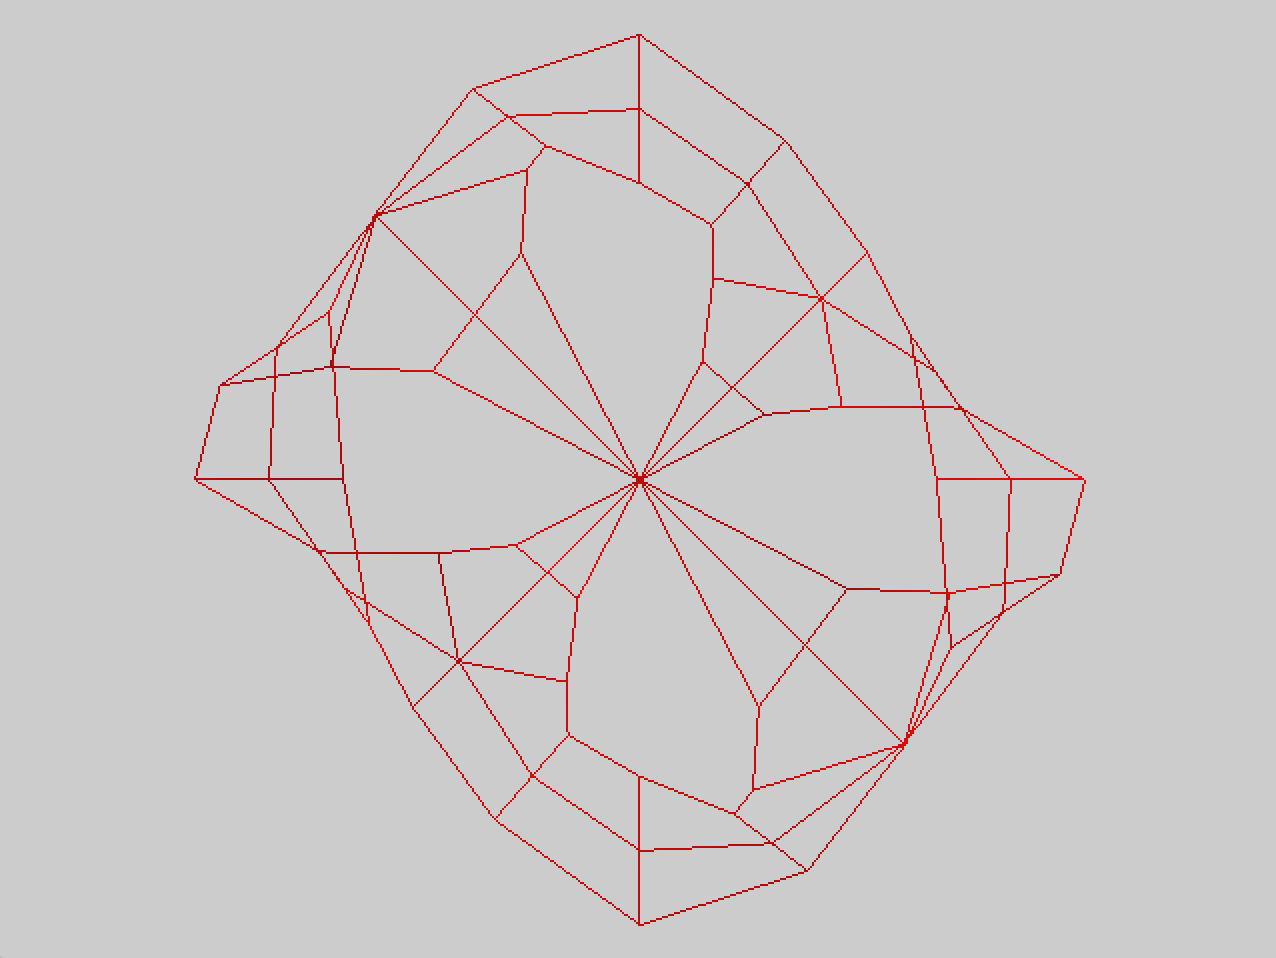
\includegraphics[width=\textwidth]{Tetra0w}
  \caption{Initial Mesh of Tetra Sculpture.} \label{figure:Tetra0}
\end{figure}

\begin{figure}[h!]
  \centering
    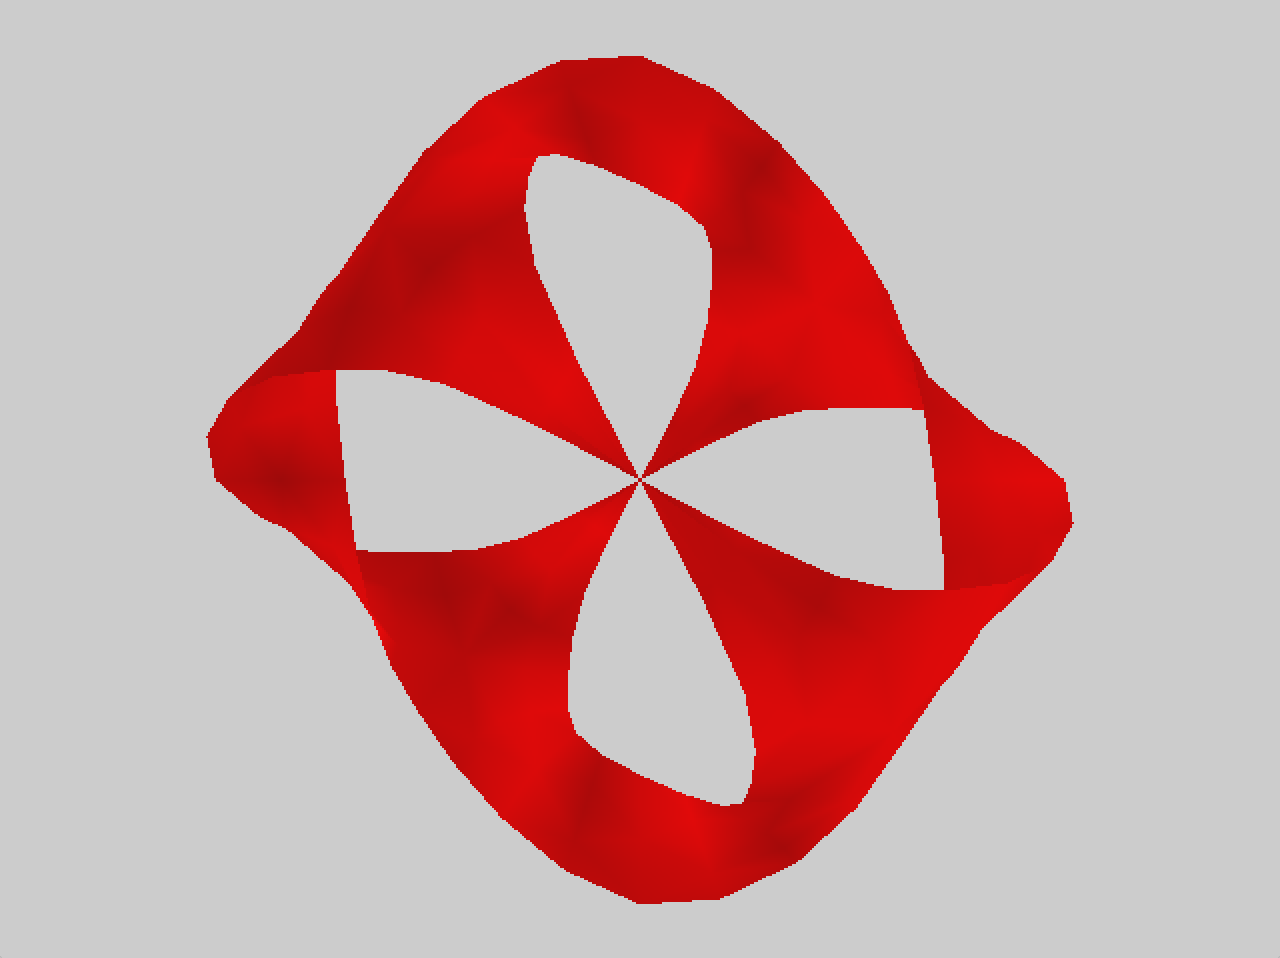
\includegraphics[width=\textwidth]{Tetra1}
    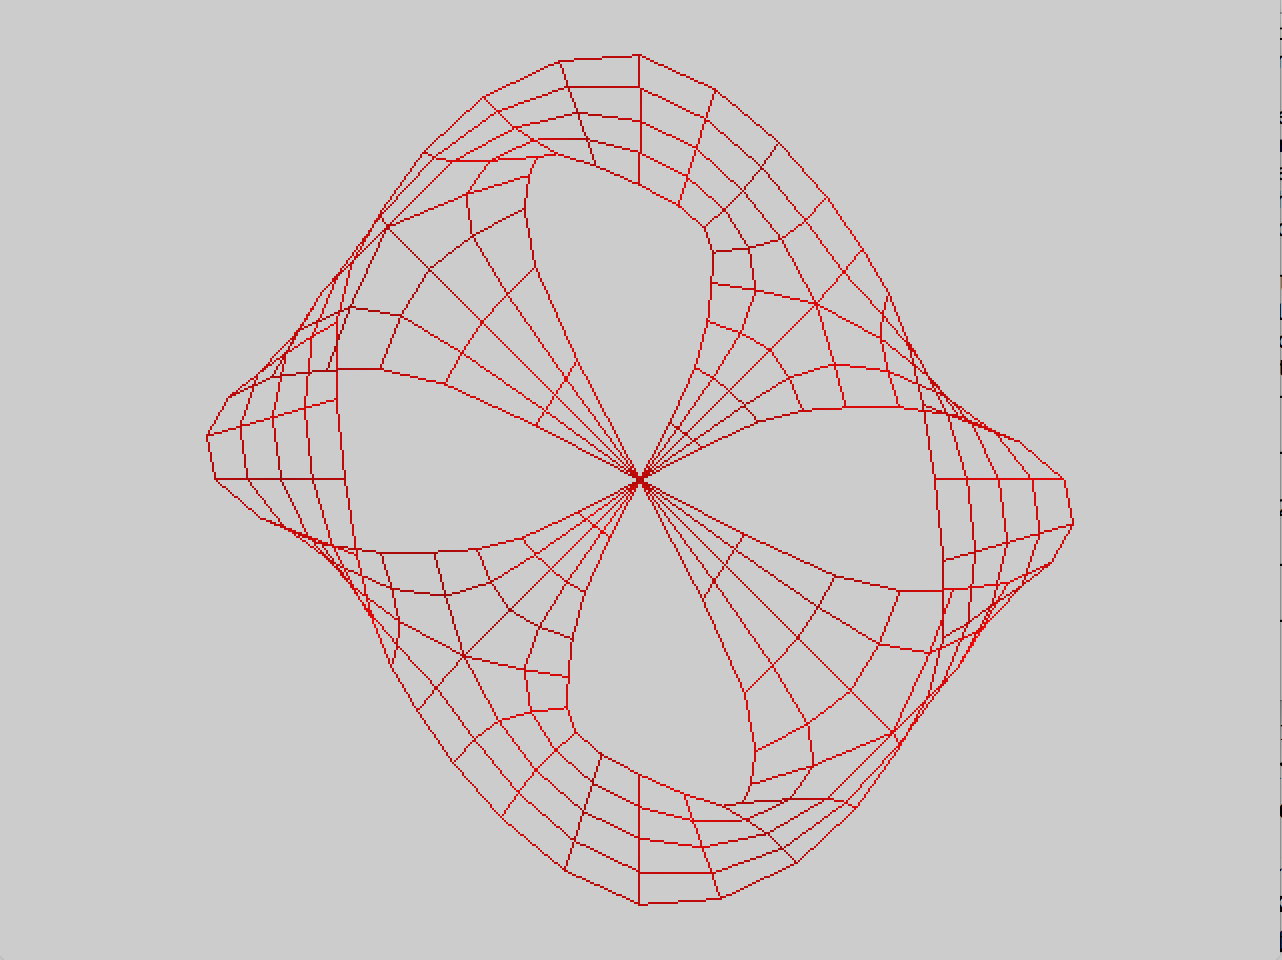
\includegraphics[width=\textwidth]{Tetra1w}
  \caption{1 Level Subdivision of Tetra Sculpture.} \label{figure:Tetra1}
\end{figure}

\begin{figure}[h!]
  \centering
    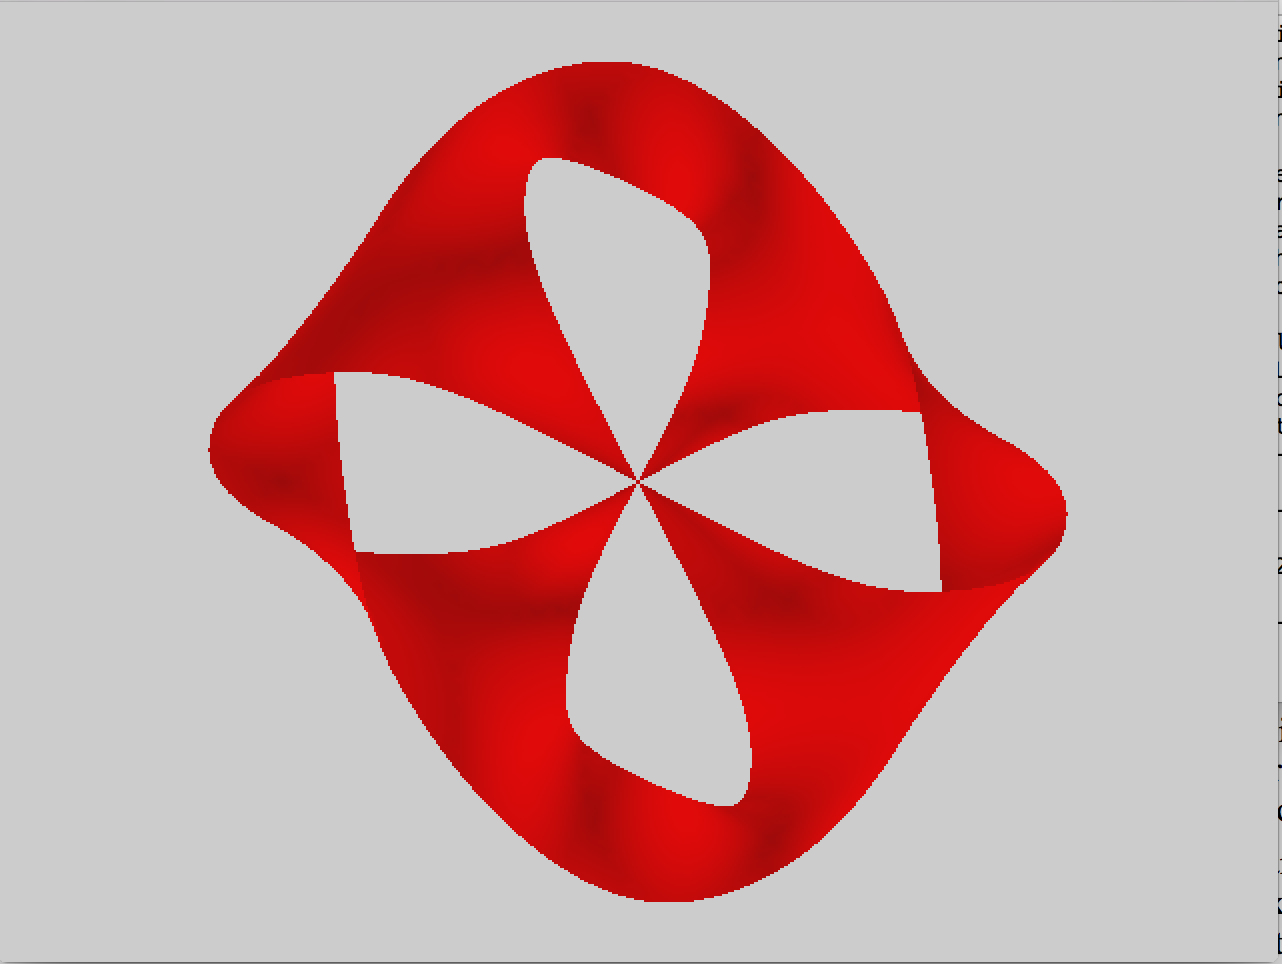
\includegraphics[width=\textwidth]{Tetra2}
    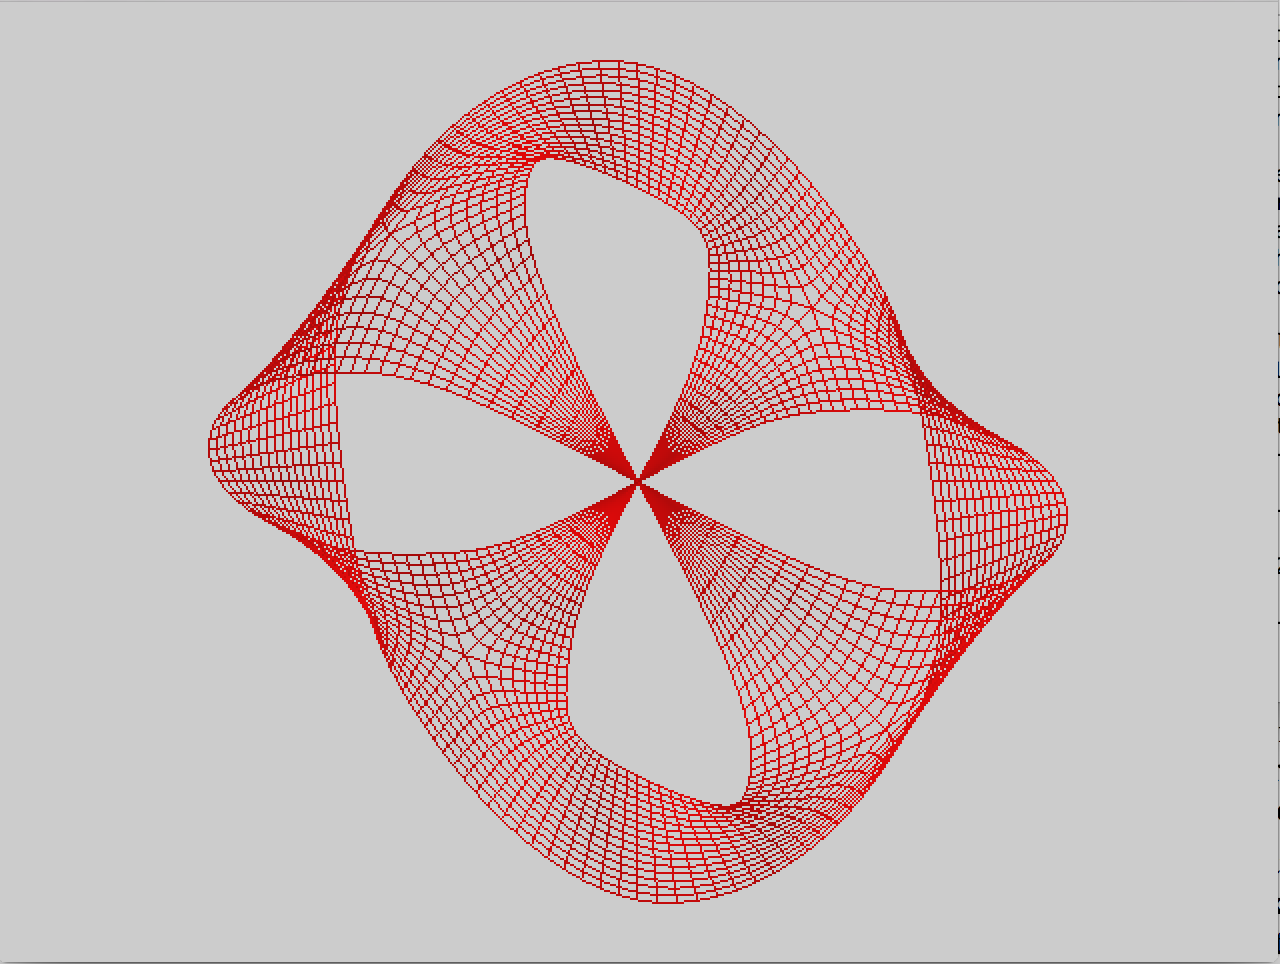
\includegraphics[width=\textwidth]{Tetra2w}
  \caption{2 Levels Subdivision of Tetra Sculpture.} \label{figure:Tetra2}
\end{figure}

\begin{figure}[h!]
  \centering
    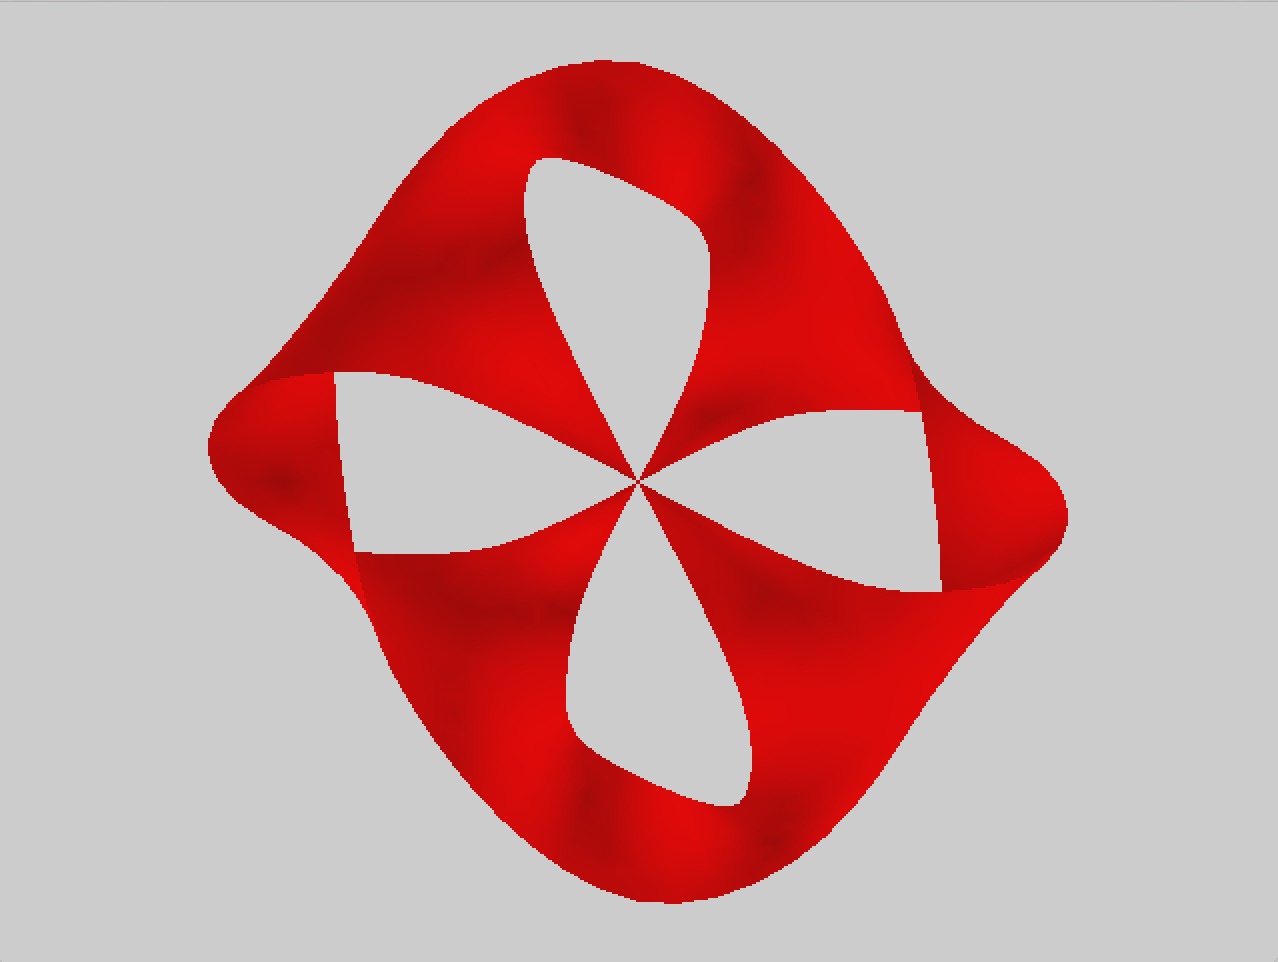
\includegraphics[width=\textwidth]{Tetra3}
    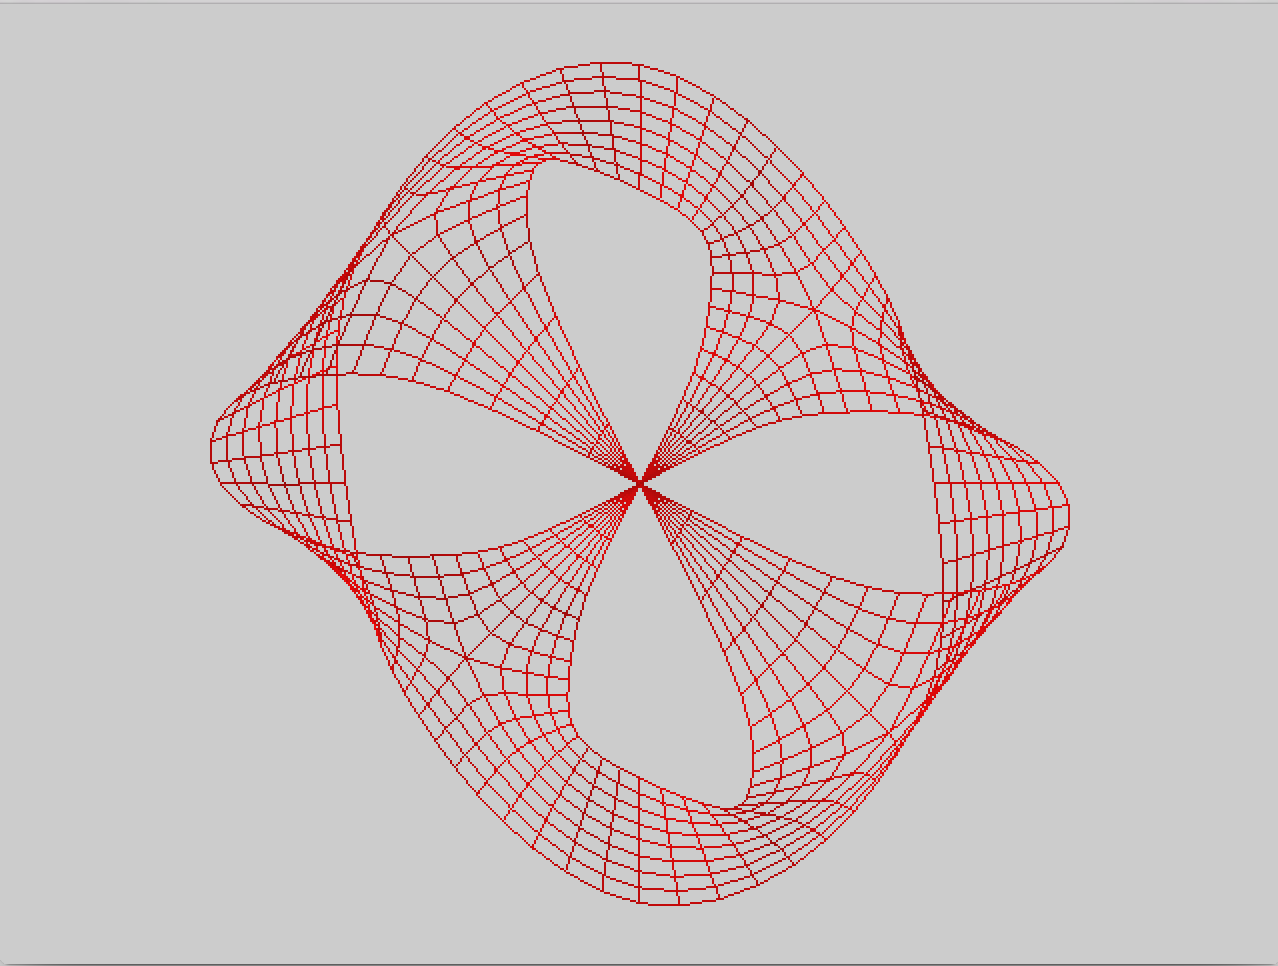
\includegraphics[width=\textwidth]{Tetra3w}
  \caption{3 Levels of Subdivision of Tetra Sculpture.} \label{figure:Tetra3}
\end{figure}

\begin{figure}[h!]
  \centering
    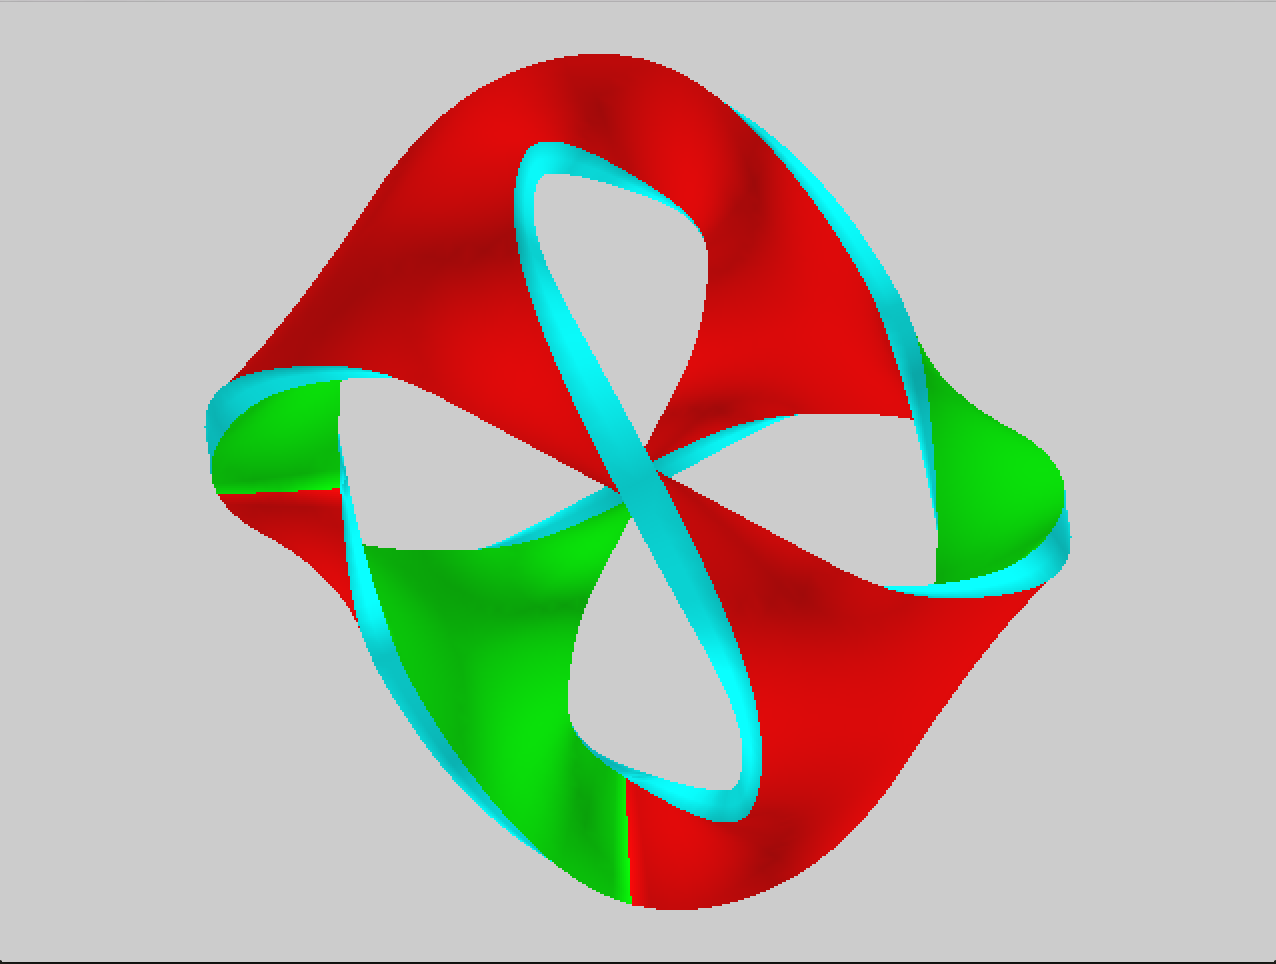
\includegraphics[width=\textwidth]{TetraOff}
  \caption{Offset after 3 Levels of Subdivision of Tetra Sculpture.} \label{figure:TetraOff}
\end{figure}

\newpage
\section{Conclusion and Future Works}
In this project, with the extended definition of halfedge data structure for single-sided surfaces, we build 1) a subdivision machine that can take in an initial polygon mesh and produce n level Catmull-Clark subdivision surface, 2) an offset machine that can take in a polygon mesh and generate offset mesh, and 3) input and output user interfaces to take in the data and display the result. It can be used to emulate sculptures and be used for the purpose of design and re-engineering.

More works would be done on the input and output end of this subdivision machine in the future. An integrated GUI will be designed to complete the following tasks: 

1) Take input with higher order geometries (e.g., funnel, tunnel, bezier curve, bspline, sweep line), and generate initial mesh for Catmull-Clark subdivision.

2) Change geometries parameters with slide bars.

3) With a better interface to display the result.

We also want to use this tool to emulate several Eva or Hild's sculptures in the future.

\end{document}
